 \documentclass[conference]{IEEEtran}
\usepackage{subfig}
\usepackage{wrapfig}
 \usepackage{amsmath}
 \usepackage{url}
 \usepackage{pifont}
 %\usepackage{times}
\usepackage{rotating}
%\usepackage{balance} 
\usepackage{color, colortbl}
\usepackage{graphicx}
\usepackage{algorithmicx}

\usepackage[running]{lineno}
\usepackage{program}
\usepackage{cite}
\usepackage{alltt}
\newcommand{\eq}[1]{Equation~\ref{eq:#1}}
\newcommand{\bi}{\begin{itemize}}
\newcommand{\ei}{\end{itemize}}
\newcommand{\be}{\begin{enumerate}}
\newcommand{\ee}{\end{enumerate}}
\newcommand{\tion}[1]{\textsection\ref{sec:#1}}
\newcommand{\fig}[1]{Figure~\ref{fig:#1}}
\definecolor{lightgray}{gray}{0.975}
\usepackage{fancyvrb}
\usepackage{stfloats}
\usepackage{multirow}
\usepackage{listings}
\usepackage{amsmath} 
\usepackage[caption=false,font=footnotesize]{subfig}
\DeclareMathOperator*{\argmin}{arg\,min} 
\DeclareMathOperator*{\argmax}{arg\,max} 


\definecolor{darkgreen}{rgb}{0,0.3,0}

\usepackage[table]{xcolor}
\definecolor{Gray}{rgb}{0.88,1,1}
\definecolor{Gray}{gray}{0.85}
\definecolor{Blue}{RGB}{0,29,193}
\newcommand{\G}{\cellcolor{green}}
\newcommand{\Y}{\cellcolor{yellow}}


\definecolor{MyDarkBlue}{rgb}{0,0.08,0.45} 
\newenvironment{changed}{\par\color{MyDarkBlue}}{\par}

\newcommand{\ADD}[1]{\textcolor{MyDarkBlue}{{\bf #1}}}
\newcommand{\addit}[1]{\begin{changed}\input{#1}\end{changed}}

\usepackage{color}
\usepackage{listings}
\usepackage{setspace}

\definecolor{Gray}{gray}{0.9}
\newcommand{\kw}[1]{\textit{#1}}
\newcommand{\quart}[4]{\begin{picture}(75,6)
  {\color{black}\put(#3,3){\circle*{2.5}}\put(#1,3){\line(1,0){#2}}}\end{picture}}
% New Commands

\definecolor{Code}{rgb}{0,0,0}
\definecolor{Decorators}{rgb}{0.5,0.5,0.5}
\definecolor{Numbers}{rgb}{0.5,0,0}
\definecolor{MatchingBrackets}{rgb}{0.25,0.5,0.5}
\definecolor{Keywords}{rgb}{0,0,1}
\definecolor{self}{rgb}{0,0,0}
\definecolor{Strings}{rgb}{0,0.63,0}
\definecolor{Comments}{rgb}{0,0.63,1}
\definecolor{Comments}{rgb}{0.5,0.5,0.5}
\definecolor{Backquotes}{rgb}{0,0,0}
\definecolor{Classname}{rgb}{0,0,0}
\definecolor{FunctionName}{rgb}{0,0,0}
\definecolor{Operators}{rgb}{0,0,0}
\definecolor{Background}{rgb}{1,1,1}

\lstnewenvironment{python}[1][]{
\lstset{
mathescape,
numbers=none,
numberstyle=\scriptsize,
numbersep=0.5em,
xleftmargin=0em,
framextopmargin=2em,
framexbottommargin=2em,
showspaces=false,
showtabs=false,
showstringspaces=false,
tabsize=2,
% Basic
basicstyle=\ttfamily\scriptsize\setstretch{0.8},
backgroundcolor=\color{Background},
language=Python,
% Comments
commentstyle=\color{Comments}\slshape,
% Strings
stringstyle=\color{Strings},
morecomment=[s][\color{Strings}]{"""}{"""},
morecomment=[s][\color{Strings}]{'''}{'''},
% keywords
morekeywords={[1]import,from,class,def,for,while,if,is,in,elif,else,not,and,or,print,break,continue,return,True,False,None,access,as,,del,except,exec,finally,global,import,lambda,pass,print,raise,try,assert, dot, norm, zip, sorted},
keywordstyle={[1]\color{Code}\bfseries},
% additional keywords
morekeywords={[3]fastmap, project, furthest, split, WHERE,clusterer, getContours, envied, fWeight, nearestContour, projection, mutate, HERE, knn},
keywordstyle={[3]\color{Keywords}\bfseries},
morekeywords={[2]@invari},
keywordstyle={[2]\color{Decorators}\slshape},
emph={self},
emphstyle={\color{self}\slshape},
%
}}{}
 
\title{Learning Actionable Analytics 
 (with applications for reducing defects and reducing runtimes)}
\author{
% You can go ahead and credit any number of authors here,
% e.g. one 'row of three' or two rows (consisting of one row of three
% and a second row of one, two or three).
%
% The command \alignauthor (no curly braces needed) should
% precede each author name, affiliation/snail-mail address and
% e-mail address. Additionally, tag each line of
% affiliation/address with \affaddr, and tag the
% e-mail address with \email.
%
% 1st. author
Rahul Krishna, Tim Menzies, Xipeng Shen\\
       \affaddr{Computer Science, NcState, USA}\\
       \{i.m.ralk, tim.menzies, xipengshen\}@gmail.com
% 3rd. author
 % use '\and' if you need 'another row' of author names
% 4th. author
\and
 Andrian Marcus\\
       \affaddr{Computer Science, UtDallas, USA}\\
       {amarcus@utdallas.edu} }


  \pagestyle{plain}
\begin{document}
  \maketitle
  
  % make the title area
  
   
  \begin{abstract}
 As business users demand more insightful
 analytics, data scientists need to change
 their tools. Instead of merely predicting 
 some result, they also need tools that generate ``plans'';
 i.e. specific suggestions on  how to change values in order to
 improve on some predicted value.
 
 This paper proposes one such planner. ``HOW'' is a 
 tool for proposing changes to independent
 variables in order to improve on 
 the predictions of the dependent variables. Unlike other approaches
 for learning optimizations to software, HOW does not require
 an underlying of the domain. Also, HOW's plans
 are designed to result in {\em minimal displacement}
 to current practice.
 
 This paper uses  HOW to learn methods
 to reduce defects and decrease program runtime.
 For the test data of this paper, the improvements generated by HERE can reduce
 defect counts as well as runtimes by up to
 50\% of their original values.
  \end{abstract}
  \begin{IEEEkeywords}
Defect prediction, configuration, prediction, planning, instance-based reasoning.
  \end{IEEEkeywords}
  
\section{Introduction}
Business  users   now demand   data mining tools
that  support a  business-level
interpretation of that data. For example,
at a  panel on software analytics at ICSE'12,
industrial practitioners lamented the state of the art in data mining
and software engineering~\cite{menzies12a}. Panelists commented that
``prediction is all well and good, but what about decision
making?''. That is, these panelists are more interested in the interpretations
and follow-up
that occurs {\em after} the mining, rather than just  the mining itself. For example:
\bi
\item Instead of just accepting  {\em predictions} on how many 
 software defects
to expect,  business users might now demand a {\em plan} to
reduce the likelihood of those defects;
\item Instead of just accepting {\em predictions} on the runtime
time of their software, business users might now demand
a {\em plan} to reduce that runtime.
\ei
In these two points, we say that a ``plan'' is a  set of proposed changes in order to better achieve some goal. 
Generating {\em plans} is a  very different task the standard
data mining tasks of {\em predicting} some discrete or numeric class.
Predictors
and classifiers only tell us what {\em is} while planners 
  tell us {\em what to change}. For the kind of business user
discussed above, planners are the preferred to mere prediction systems
since, as one gruff user once shouted at us:
\begin{quote}
{\em ``Don't tell me what \underline{is};
tell me what to \underline{change}.''}
\end{quote}
Generating plans is also differed to the recommender systems. 
discussed by Robillard and Walker~\cite{rob14}.  Recommendor systems
in software engineering
are less {\em directive} and more    {\em collaborative} than plan generators:
\bi
\item
Directive systems (such as those discussed in this paper) tell developers exactly what to do;
e.g. ``use these settings in a Makefile''. 
\item
On the other hand, the collaborative systems discussed by Robillard and Walker
are more suggestive guides that
help (e.g.) programmers focus on very small sets
with  very large libraries of code of documentation.
\ei
This paper presents HOW, a novel planner for learning actionable analytics.
In the experiments shown below, we see that HOW's plans can
significantly reduce the expected
value of:
\bi
\item The software defects found in  the object-oriented JAVA systems explored in 2010 by Jureczko et al.~\cite{jureczko10};
\item The runtime of the  software systems whose configurations
are explored in 2013 by Seigmund et al.~\cite{sven12};
\ei
In summary, this paper makes five contributions that are significantly different to
prior work:
\be
\item The HOW  instance-based planner of this paper has not been presented before.
\item The experiments of this paper show that HOW planner is useful for real-world tasks;
e.g. reducing the
expected values of the Jureczko software defects and the Seigmund software runtimes.
\item Apart from HOW, we  also offers a general framework for using  predictive system to build planners;
\item Further, we offer a  test to recognizes  when we should {\em not}  plan: specifically,
planning is
not recommended in domains with  poorly performing predictors;
\item Last, we  offer a general verification rig for assessing the value of plans generated within this rig.
\ee
The rest of this paper is structured as follows.
HOW's instance-based reasoning  makes its conclusions by
studying the space of examples. As discussed in \tion{mm},
this is a very different approach to
{\em model-based planners} that use the model
as sub-routine within a Monte Carlo simulation~\cite{me07f} or the evolutionary 
programming methods explored by the search-based software
engineering community~\cite{krall14,harman12dec}.  
 
 

\section{HOW: Motivation and Methods}\label{sec:mm}
 
 \subsection{Motivation: Why ``HOW''?}
HOW was inspired by two     business issues raised about the  GALE optimizer~\cite{krall14}. 
A well-known effect in machine learning (and, in computer vision
and compression~\cite{levina04}) is that the $n$ dimensions of a data set can be represented by a  much
lower-dimensional approximation. GALE finds those $m \ll n$ dimensions then mutates examples
towards the better end of each dimension $m_i$. Since it explores $m \ll n$ dimensions,
GALE terminates much faster than standard optimiser (e.g. for one large model, 4 minutes versus 7 hours~\cite{krall14}).
Better yet, GALE's rapdily generated  solutions are competitive (or better) than those found by 
slower optimizers.

When GALE executes, it searches for better examples of data
 by (a)~inputting an initial population of data; then (b)~making
 extensive mutation to that data. In practice, GALE makes
100s to 100,000s of mutations. Each of these mutations
is reassessed using some domain model.
For certain users,this approach raises some issues.  One such user commented:
\begin{quote}
ISSUE~\#1: {\em ``What if I only want the minimum useful change, not
the maximum possible?''}
\end{quote}
Note here that this business user is asking for solutions  that do not require extensive 
changes to their current  approaches. 

Later in that discussion, another business user asked:
\begin{quote}
ISSUE~\#2: {\em ``But what if I do not have a domain model of my business?''}
\end{quote}
This also is a legitimate issue.
Building and certifying a model  can  takes  long time, especially in software engineering. For  example, in previous work~\cite{me07f} we used models
developed by Boehm's group at the University of Southern California.
Some of those models took decades to develop and mature (from 1981~\cite{boehm81} to 2000~\cite{boehm00b}). 

Also, even when there is an existing model, they can require
constant  maintenance lest they become out-dated. Elsewhere, we have described our
extensions to the USC models to enable reasoning about agile software developments. 
It took many months to implement and certify those extensions~\cite{me09i,me09j}.
The problem of model maintenance is another
motivation to look for alternate methods that can be automatically updated whenever new data arrives.

Further, sometimes  it is easier to access instances of a model's behaviour than the model
itself. For example, in prior work with Martin  Feather from the Jet Propulsion 
Laboratory~\cite{fea02a},  our research partner could not share a
propriety model from within the NASA firewalls. However, they could share 
logs of the input/output of that model.
 
These two issues are not just problems for GALE, but also for every
other model-based optimization algorithm  that makes
extensive use of mutation  and domain models such as
NSGA-II, NSGA-III, SPEA2, IBEA, PSO, DE, MOEA/D, etc.~\cite{deb00a,zit02,zit04,%
deb14,Cui2005a,storn97,zhang07:TEC}. Accordingly, this paper seeks
an optimization methods that make minimal changes to instances,
while avoiding the problem of models that are missing, slow
to build, hard to maintain, or difficult to access.

\subsection{Methods: How to Build ``HOW''?}

A general model for {\em predictors} is as follows. 
During testing, each test instance gains a prediction 
by finding which region of the data it falls into.
During training, those regions are inferred from
divisions that ``chunk'' together regions with instances
with similar properties. These dividers can be categorical (as in the case of decision trees) or probabilistic (as in the
case of Naive Bayes) or learned via some distance minimization
process 
(as in the case of support vector machines) or generated
directly by some clustering algorithm. 


\begin{figure}[t!]
\small
~\hrule~

{\bf \fig{where}a: top down clustering:}

Data can be rapidly and recursively divided   as follows.
Find   two   distance instances,  $X,Y$
by picking any instance $W$ at random, then setting $X$ to its most
distant instance, then setting $Y$ to the instance most distant from
$X$~\cite{fastmap}
(this requires only $O(2N)$ comparisons
of $N$ instances).
Next, project each instance $Z$
onto a line that  runs between $X,Y$ using the cosine
rule of \fig{where}b. After that,  split the data at the median $x$ value of all instances and
recurses on each half  (stopping when
one half has less  than $\sqrt{N}$ of the original population). See \fig{code1d} for further details.

~\hrule~
 
{\bf \fig{where}b: finding distances:}

In the \fig{where}a, to compute distances, we use
the Euclidean measure recommended for
instance-based reasoning by Aha et al.~\cite{aha91};
i.e. $\sqrt{\sum_iw_i(X_i-Y_i)^2}$ where $X_i,Y_i$
where values are  normalized 0..1 for the range min..max and 
$w_i$ is some importance weight given to attribute $i$.
Usually, $w_i=1$ but it can be adjusted using, say,
the feature weighting methods of \fig{where}d.
 
 ~\hrule~
 
{\bf \fig{where}c: 3 point geometry:}
 
Let   $X,Y$ be two points joined by  a line  length $c$.
A third point, $Z$, has distances  $a=dist(Z,X)$ and
$b=dist(Z,Y)$ to $X,Y$, respectively.
According to the cosine rule,   $Z$ projects onto  $\overline{XY}$
at distance $x=(a^2 + c^2 - b^2)/(2c)$ from $X$.
Further, according to Pythagoras' theorem, $Z$ stands at a distance
$y = \sqrt{a^2 - x^2}$ from the line $\overline{XY}$. See \fig{code1c} for further details.

~\hrule~

{\bf \fig{where}d: feature weighting:}

HERE's feature weighting algorithm
comes from the CART regression tree learner~\cite{Breiman1984}.
It sorts independent variables
 according to how well they can reduce the variance
of a  numeric objective.
If we split some column $i$ of independent numeric data  into $N=n_1 + n_2 + ..$ splits,
then the expected
value of the objective value of the split  is $w_i = \sum_i v_in_i/N$
where $v$ is the standard deviation of the objective.
A recursive procedure can  find those divisions $n_1,n_2,...$ by (a)~sorting a numeric column,
then split at $\argmin_i w_i$, then recursing into each half.  See \fig{code1d} for further details

~\hrule~
 
\caption{Sub-routines within HOW.}\label{fig:where}
\end{figure}



\begin{figure} 
\begin{python}[right]
def HERE(trainingData, testingData):
  training(trainingData)
  return [nearest(z).displace(z) 
          for z in testing]

def training(trainingData):
  Line.using = what2Use(trainingData)
  clusters = cluster(trainingData):
  for cluster in clusters:
    one = examplar(cluster)
    two = examplar(nearest(one, clusters))
    Line(one,two)
  
def what2Use(trainingData):
  second  = lambda lst: lst[1]
  weights = map(second,
                sorted(featureWeighting(trainingData)))
  use    = int(len(weights)*Line.B)
  return [i for i,_ in enumerate(weights[:use])]

def nearestLine(z):
  out,least=None,10000
  for line in Line.all:
    d = line.dist(z)
    if d < least: out,least = line,d
  return out
\end{python}
\caption{Instance-based Planning using HERE.
Testing data is {\em displaced}
towards   the $X$ point of the nearest {\tt Line} (defined in \fig{line})
The {\tt geometry} method comes from \fig{code1c}.
The {\tt featureWeighting} function comes from \fig{code1a}.
The {\tt cluster} function comes from \fig{fastmapCode}.
}\label{fig:HERE}   
\end{figure}



\begin{figure} 
\begin{python}[right]
class Line:
  "Lines connect a worse cluster Y to a better one X"
  all   = []
  using = []
  F     = 0.5
  B     = 0.5
   def __init__(i,x,y):
    if x.score < y.score:
      x,y = y,x
    i.c = dist(x,y) 
    i.obj = len(x) 
    Line.all += [i]
  def displace(i,z):
    for j,(xj,zj) in enumerate(zip(x,z)):
      if not j == i.obj and  j in Line.using:
         z[j] = zj + Line.F*( xj. - zj
    return z
  def dist(i,z):
    _,out = geometry(i.x,i.y,z)
    return out
  def exemplar(i,cluster):
    #Apply the rules at end of section II.B
\end{python}
\caption{The primary data structure of HOW
is the {\tt Line}.
Training data is converted into a set of {\tt Line}s,
each of which is defined by a $X,Y$ pair, where $X$
has better scores than $Y$. }\label{fig:line}
\end{figure}




\begin{figure} 
\begin{python}[left]
def dist(x,y):
   "See Aha et al. reference [22]. XXX"
   
def geometry(x, y, c, z): 
  a = dist(z,x)
  b = dist(z,y) 
  x= $(a^2 + c^2 - b^2)/(2ac)$ 
  y=  $\sqrt{a^2 - max(x,0)^2)}$
  return x,y
  
def nearest(x,data):
  return furthest(x,data,best=1000,better=lt)
 
def furthest(x,data, best= -1, better=gt):  
  out = None
  for one in data:
    d = dist(one,x)
    if gt(d,best): out, best = y, d
  return out
\end{python}
\caption{Some routines for 3 point geometry,  from \fig{where}.c.}\label{fig:code1c}
\end{figure} 


\begin{figure}
\begin{python}[left]
def featureWeighting(cols):
   obj = len(cols[0])
   return sorted(weight1(col,i,obj) 
                for i,col in enumerate(cols)
                if not i == obj)

def weight1(i,obj,col):
  pairs = sorted([row[i],row[obj] for row in col])
  n     = length(col)
  return sum(v*n1/n for v,n1 in recurse(pairs,[])),i

def recurse(this,cuts):
  cut,sd = divide(this)
  if cut:
    recurse(this[:cut],cuts)
    recurse(this[cut:],cuts)
  else:
    cuts += [(sd,len(this)]
  return cuts
    
def divide(this,tiny=2):
  lhs, rhs = Stats(), Stats(x[1] for x in this)
  n, least, cut = rhs.n*1.0, rhs.sd(), None
  for j,x in enumerate(this):
     if lhs.n > tiny and rhs.n > tiny:
       tmp = lhs.n/n*lhs.sd() + rhs.n/n * rhs.sd()
       if tmp < least:
          cut,least = j,tmp
     rhs - x[1]
     lhs + x[1]
  return cut,least
  
class Stats():  
    def __init__(i,inits=[]):
      i.n = i.mu = i.m2 = 0.0
      map(i.__add__,inits)
    def sd(i) :  
      return (max(0.0,i.m2)/(i.n - 1))**0.5
    def __add__(i,x):
      i.n  += 1
      delta = x - i.mu
      i.mu += delta/(1.0*i.n)
      i.m2 += delta*(x - i.mu) 
    def __sub__(i,x):
      i.n  -= 1
      delta = x - i.mu
      i.mu -= delta/(1.0*i.n)
      i.m2 -= delta*(x - i.mu) 
\end{python}
\caption{Feature weighting, from \fig{where}.d.}\label{fig:code1a}
\end{figure}

\begin{figure} 
\begin{python}[left]
def cluster(data, n,lvl=100):
  if lvl < 1: 
     return data # stop if out of levels
  leafs = [] # Empty Set
  x,y,left,right = splitAcross2Points(data) 
  if len(left) > $\sqrt{n}$:  
     leafs += cluster(left, n, lvl - 1)  
  if len(right) > $\sqrt{n}$:  
     leafs += cluster(right,n,  lvl - 1) 
  data.has = dict(x=x,y=y,
                 l=left,r=right,
                 leafs=leafs)
  return leafs
  
def splitAcross2Points(data): 
  tmp = random.choose(data)
  x = furthest(tmp, data)
  y = furthest(x, data) 
  c = dist(x,y)  
  if x.scores < y.scores:
     x,y = y,x 
  for one in data.members: 
    one.pos = geometry(x,y,c,one)
  data = sorted(data) # sorted by 'pos.x'
  return x, y, split(data)
  
def split(data):   
  mid = len(data)/2; 
  return data[mid:], data[:mid]
\end{python}
\caption{Clustering. Lines 16,17,18 come from~\cite{fastmap}. }\label{fig:fastmapCode}   
\end{figure}




Those same regions can be used for instance-based 
{\em planning}-- but instead of leaving test instances in the regions
found during training, we {\em displace} them towards regions
with better objective scores.
To achieve this, 
during training, HOW clusters data using the procedure of \fig{where}a,
then draws lines between the centroids of  clusters $X,Y$ that are nearest
neighbors.
By convention, we say that the cluster containing $X$ has the  better objective scores. This means we can say that the line is a useful direction for displacing
data; i.e.  away from $Y$ and towards $X$.
Hence,  during testing,  HOW use Pythagoras' theorem
and \fig{where}c to find the  nearest line to every test instance. That test instance is   then displaced towards the better end
of that line (towards  $X$).

An important design decision with HOW 
is how to determine the exact {\em direction} and {\em magnitude} of the
displacement.  Following on from the discussion around   ISSUE~\#1,
we note that a design goal of HOW is
{\em minimal displacements} of project data.
To implement minimal displacement:
\bi
\item
HOW sorts  the independent variables
using the procedure of  \fig{where}d. It then only
displaces the    best $B$\%  of that sort (while leaving the rest untouched).
In  the experiments shown below,  we explore   $B \in \{25,50,100\}\%$.
\item
HOW also  limits displacement
to very small regions in the space of the training data (never more that the separation
of the two closest clusters).  HOW's clusterer divides  data into many   small clusters containing
$\sqrt{N}$ of the population.
HOW   limits displacement to  \mbox{$0 \le F \le c$}, where
$c$ is the distance between the two closest clusters. 
In  the experiments shown below,  we explore
\mbox{$F\in \{0.25, 0.5, 0.75\}$}.
\ei
Turning now to the displacement {\em direction},
our experiments show that it useful to  carefully reflect on exactly where HOW should  push each test instance.
HOW replaces each cluster   with one {\em exemplar} that best
characterizes the data in that cluster. It then displaces the
test data towards that exemplar, as follows.
Let $Z_j$ be an independent variable within the
test instance $Z$. If  $X$ be the exemplar found at training time,
then we displace $Z$ as follows:
\[Z_j =  Z_j + F*(X_j - Z_j)\]
Here, $F$ is the  magnitude controller, discussed above.
The experiments of this work showed that different kinds of data require
different kinds of exemplars.
\bi
\item
For the Seigmund data,
the objective score is the runtime of the test suite of a compiled program.
For this kind of data with numeric objectives,
the exemplar  is the instance in a cluster
with  best objective score.
\item
For the Jureczko data, the objective score
is a boolean that is true if defects have been noted
for that class. 
For this kind of data with discrete objectives,
the data, 
has less differentiation between the objective scores
so we set the exemplar to  
an instance synthesized from the median values of the instances
in that cluster.
\ei 

  
  
\begin{figure}[!t]
\small 
\[
\begin{array}{r}
\mathrm{project}\\
\mathrm{data}
\end{array} 
\left\{\begin{array}{l}\mathit{train}
        \left\{\begin{array}{l}
                \mathrm{learn\;a\;}\mathrm{predictor\;}\mathrm{(e.g.\;via \;Random\;Forest)}\\
                \mathrm{learn\;a\;}\mathrm{planner\;}\mathrm{(e.g.\;via \; HOW)}
              \end{array}\right.
       \\
      ~\\
\mathit{test}  
    \left\{\begin{array}{l@{~}l}
           \mathit{before}& =\mathrm{predictor}(\mathit{test})\\
           \mathrm{\bf if\;}\mathit{before} & <  \mathit{satisfactory}\\
           \mathrm{\bf then}  & \mathrm{{\bf return}\; 0}\\~\\
           \mathrm{\bf else} &
           \left\{
            \begin{array}{l}
                \mathit{test'} = \mathrm{planner}(\mathit{test})\\
                \mathit{after} =\mathrm{predictor}(\mathit{test'})\\ 
                \mathrm{{\bf return}\;} \mathit{after} /  \mathit{before}
            \end{array}
          \right.
   \end{array}\right.
\end{array} \right. 
\]
 
\caption{How to use {\em predictors} for {\em planning}.}\label{fig:work}
\end{figure}



\subsection{How to Assess ``HOW''}
In the experiments shown below,  HOW comments  on how to reduce
software defects by adjusting certain static code parameters of the code\footnote{Such parameters can be manually adjusted by programmers or (for large scale changes) automatically adjusted using code refactoring
tools, as shown by Binkely et al. in 2006~\cite{Binkley2006} and more recently by Mkaouer et al. in 2015~\cite{Mkaouer15}.}. How are we to verify that HOW's recommendations actually work? 

Some organizations have the resources to 
run repeated trials to assess the effect of different treatments.
For example, in one remarkable recent study, Bente et al. report results
were the same specification was developed into a product by four different organizations~\cite{Anda2009}. Given those kind of resources, it would be possible
to (say) take a code base, assign it to $N$ different teams, apply
HOW's plans the code used by  $N/2$ teams, then check in 12 months time
if those halves of the teams have fewer defects than the other.  

Very few industrial or research groups have access
to the kinds of resources using by Bente et al. (evidence: in the size years since the
publication of that work, we know of only one of two similar studies). Hence, it
we wish to verify HOW's plans, then some other framework is required that is less
resource intensive.
 




We propose using prediction systems (built by data mining) as a verification
tool for planners. In domains with data, from which data miners can build
predictors of adequate performance, then those predictors can assess the value
of the changes proposed by HOW.

As shown in \fig{work}, our proposal divides
project data  into two disjoint sets {\em train} and {\em test}
(so \mbox{{\em train} $\cup$ {\em test} $=\;\emptyset$}).
Next, from the train set, we build both a {\em planner} as well
as a {  predictor}. Our general framework does not   commit to any particular  choice
of { planner} or { predictor} but, for the purposes of this paper, 
our { planner}
will be HOW  and our
our { predictors} will be the Random Forest and Random Forest
Regressor taken from the SciKit
Learn toolkit~\cite{Pedregosa2012}. The Random Forests procedure is explained in \fig{rr}. 

\begin{figure}[t!]
\small
\begin{tabular}{|p{.95\linewidth}|}\hline
 Decision tree learners find the attribute whose value's
select for for sections of the data with least variation in the class
variable. Decision tree learners then recurse on each selection~\cite{breiman84}. 

A random forest is a set of decision trees, each built
from some random subset of the rows and columns. The conclusions
of the forest are a ``vote'' generated by all the trees~\cite{Breiman2001}. 

A standard Random Forest predicts for a discrete class variable while
a Random Forest Regressor generates numeric predictions.\\\hline
\end{tabular}
\caption{Random Forests and Random Forest Regressors.}\label{fig:rr}
\end{figure}


Turning now to the {\em test} data, this is passed to the { predictor}
to generate a baseline {\em before} performance score.
Note that if our { predictors} fail to perform adequately on the test data,
then we cannot trust them to comment on our plans. Accordingly,
if that performance is unsatisfactory, we abort.
Else, we (1)~apply the { planner} to alter the {\em test} data;
then (2)~apply the { predictor} to the altered data {\em test'};
then (3)~return the performance delta.




\begin{figure*}[!t]
\scriptsize
   \begin{center}
   \begin{minipage}{.46\linewidth}
    \begin{tabular}{r@{~}|l@{~}|r@{~}|l@{~}|r@{~}|r@{~}|} \cline{2-6}
   & \multicolumn{5}{c|}{ }\\ 
   
   & \multicolumn{5}{c|}{ Data set  properties}\\ 
   & \multicolumn{5}{c|}{  }\\ 
           & \multicolumn{2}{c|}{training}   & \multicolumn{3}{c|}{testing}      \\ \cline{2-6}
   data set      & versions           & instances & versions     & instances    & \% defective             \\ \hline
        jedit    & 3.2, 4.0, 4.1, 4.2 & 1257      & 4.3          & 492          & 2 \\
        ivy      & 1.1, 1.4           & 352       & 2.0          & 352          & 11 \\
        camel    & 1.0, 1.2, 1.4      & 1819      & 1.6          & 965          & 19 \\
        ant      & 1.3, 1.4, 1.5, 1.6 & 947       & 1.7          & 745          & 22 \\
        synapse  & 1.0, 1.1           & 379       & 1.2          & 256          & 34 \\
        velocity & 1.4, 1.5           & 410       & 1.6          & 229          & 34 \\
        lucene   & 2.0, 2.2           & 442       & 2.4          & 340          & 59 \\
        poi      & 1.5, 2, 2.5        & 936       & 3.0          & 442          & 64 \\
        xerces   & 1.0, 1.2, 1.3      & 1055      & 1.4          & 588          & 74  \\ 
        log4j    & 1.0, 1.1           & 244       & 1.2          & 205          & 92   \\
        xalan    & 2.4, 2.5, 2.6      & 2411      & 2.7          & 909          & 99  \\\hline
        \multicolumn{6}{c}{~}\\
        \multicolumn{6}{c}{~}\\
        \multicolumn{6}{c}{~}\\
        
        
    \end{tabular}\end{minipage}\begin{minipage}{.4\linewidth}
    \begin{tabular}{|rrr|rrr|rr|l} \cline{1-8}
      \multicolumn{8}{|c|}{  }\\
      \multicolumn{8}{|c|}{  Results from learning}\\
       \multicolumn{8}{|c|}{   }\\
   \multicolumn{3}{|c|}{untuned} & \multicolumn{3}{c|}{tuned} & \multicolumn{2}{c|}{change}\\
  \cline{1-8}
  
  pd & pf & good? & pd & pf & good? & pd & pf\\\cline{1-8}
  50 & 27 &   & 64 & 28 & y & 14 & 1&$\star$\\
  65 & 35 & y & 65 & 25 & y & 0 & -10&$\star$\\
  50 & 30 &   & 62 & 41 &   & 12 & 11\\
  66 & 21 & y & 63 & 18 & y & -3 & -3\\
  45 & 18 &   & 47 & 15 &   & 2 & -3\\
  79 & 61 &   & 77 & 61 &   & -2 & 0\\
  55 & 25 &   & 60 & 27 & y & 5 & 2\\
  51 & 32 &   & 61 & 12 & y & 10 & -20&$\star$\\
 30 & 28 &   & 39 & 33 &   & 9 & 5&$\times$\\
  32 & 6 &   & 30 & 9 &   & -2 & 3&$\times$\\
  41 & 5 &   & 48 & 0 &   & 7 & -5&\times\\
\hline
  \multicolumn{5}{c}{~}    &  & -1 & -4& 25th\\
\multicolumn{6}{r|}{the percentiles of the changes:}    &   5 & 0 & 50th\\
 \multicolumn{5}{c}{~}             & & 10 & 3 & 75th\\
\end{tabular}

\end{minipage}
\end{center}    
  
    \caption{Training and test {\em data set properties} for the Jureczko data sets,
    sorted in ascending order of \% defective examples.
    On the right-hand-side, we show the {\em results from learning}.
    Data is ``good'' if it has   recalls over 60\% and false alarms under 40\%
(and note that, after tuning, there are more ``good'' than before).
Data   marked with ``$\star$'' show large improvements in performance, after tuning.
Data   marked with ``$\times$'' are not ``good'' since their test suites  have so few undefective examples (less than 5\% of the total sample) that it becomes harder to find better data towards which we can displace test data.
}\label{fig:j}
\end{figure*}


\section{When Not to Plan: \\the Problem of Poor Predictors}

The clear advantage of the approach of \fig{work} is that it can be readily and automatically
applied to domains with historical data. That said, the obvious drawback with this approach
is that our assessment of the plans is only as good as the predictor. To 
mitigate for this {\em problem of poor predictors}, it is hence wise to demand certain standards for the {\em
satisfactory} threshold used in this \fig{work}. 
 

For example, this study's data from two types of domains: the Jureczko   object-oriented data  
and the Seigmund configuration data. 
For the Seigmund data, the plans generated by HOW advise on how  to change the   configurations settings within a Makefile
(in order to make resulting compiled
code  run faster). Here, performance can be measured in terms of  difference
between the predicted runtime $p$ of test case items and their actual runtimes $a$
using  $s= 100*(1- \frac{abs(a - p)}{a})$.
This paper  explores    six Seigmund configuration data sets:  Berkeley DB (Java and Windows versions), Apache, SQLite, LLVM, and
  x264\footnote{Available from the performance prediction section of PROMISE
  http://openscience.us/repo/performance-predict.}. 
  After splitting that data into equal sized train:test groups, a Random Forest
  Regressor trained on one half, then applied to the other, achieved nearly perfect scores of
%issue 24
\[s=\{99.9, 99.8, 99.4, 99.1, 96,1\}\]
That is, we can be very confident that the predictors from the Seigmund data can assess
HOW's plans.
(Aside: if the reader doubts that such high scores are achievable, we note that these scores are 
consistent with those achieved by predictors built by Seigmund et al.~\cite{sven12}.)

Turning now to the Jureczko   OO data sets, we found:
\bi
\item
Most   predictors in this domain were far from      perfect;
\item 
But several of these predictors could
be salvaged using some sampling and optimization methods (see the notes on SMOTE and differential evolution, below).
\ei
As shown in \fig{j}, we   explore numerous examples of the Jureczko   object-oriented static code data sets: Ant, Camel, Ivy, Jedit,   Log4, Lucene, Poi, Synapse, Velocity, Xalan, Xerces\footnote{Available from the object-oriented defects section of the PROMISE respository openscience.us/repo/defect/ck.}. 
Given access to $V$ released
versions, we test on version $V$ and train on the available data from earlier releases (as
shown in \fig{j}, this means that we are training on hundreds to thousands
of classes and testing on smaller test suites).
Note the three bottom rows marked with $\times$: these contain predominately
defective classes (two-thirds, or more) and in such data sets, it is hard to distinguish
good from bad (since there are so many bad examples). 

For the  Jureczko   data,
the plans generated by HOW advise   how to change static code attributes in order to reduce defects in
Java classes.  Here,
performance can be measured in terms of:
\bi
\item Probability of detection (a.k.a. ``pd'' or recall) which is the percent of faulty classes in
the test data detected
by the {\em predictor}.
\item Probability of false alarm (a.k.a. ``pf'') which is the percent of non-fault
classes that are predicted to be defective.
\ei 
The ``untuned'' columns of \fig{j} shows RandomForest's learned {\em pd,pf}
values generated after learning from the training data, then being applied to the test data.
If we define ``good'' to mean $\mathit{pd}>60 \wedge \mathit{pf} < 40$\%,
then only two of our data sets ({\em ivy,ant}) are ``good'' enough. 

The ``tuned'' columns of \fig{j} show that we can salvage some of the data sets
using two techniques.
 Pelayo and Dick~\cite{pelayo07} report that defect prediction can be improved via SMOTE~\cite{Chawla2002}; i.e. an over-sampling of minority-class examples.
 Also, Fu et al.~\cite{fu:ase15} report that an optimization method called differential evolution~\cite{storn97}
applied to defect predictors can quickly explore the tuning
options of Random Forest to find better settings for the size of the forest, the termination criteria
for tree generation, etc.
The rows marked with $\star$ in \fig{j} show data sets whose performance was improved remarkably by these
techniques. For example, in {\em poi}, the recall increased by 10\% while the false alarm rate dropped by 20\%).
However,  as might be expected
the the three bottom rows remain
unsalvageable.

In summary, while we cannot trust predictors from some of our data sets,
we can plan ways to reduce defects in {\em jedit, ivy, ant, lucene} and {\em poi}.
(Aside: note that this tuning used optimization and sub-sampling   on   {\em only} the
training instances of \fig{j}
i.e.
no clues from the test set were ever used in this tuning process.)


 
 

\section{Experimental Methods}

blah blah data. algorithms. statistics

\section{Releated Work}

Our prior work in generating policies relied upon a Monte Carlo
analysis of an underlying model~\cite{me07f}. This approach had three major problems.
Firstly, enough domain knowledge had to be collected to build that model
and this can take a long time. For example, in our previous work we used three software process models from
the Unviersity of Southern California that were initially
developed and updated for nearly two decades from 1981~\cite{boehm81} to 2000~\cite{boehm00b}.

Secondly, there is the computational cost of running those models.
While 

~\cite{}-- which suffered from the problem of (a)~the effort required to collect the domain knowledge to build
problem in certifying the underlying model;
 (b)~the computational problem of running that model enough
times to learn patterns in that data; and (c)~ requrearea used large scale simulations or large


While
our case studies are defect and runtime reduction, HERE is a general
purpose algorithm that could be applied to any table of data with at least
one column whose values can be sorted from ``desired'' to ``undesired''.



{\bf RQ1: Can Instance-based Learning techniques be used to create Planning tools that can better analyse software defect?} 


{\bf RQ2: Can lessons learnt from local policy generators be useful for generating solutions that can be used to mitigate defects in software systems?} 

{\bf RQ3: Can such instance-based planners be applied to other software engineering paradigms?}
We check if the proposed instance-based planner is applicable to performance prediction.

\section{Motivating Example}
\section{Background}
\section{Instance Based Learning}

Assessing the quality of solutions to a real-world problem can be extremely hard~\cite{menzies2005xomo}. In several software engineering applications, researchers have models that can emulate the problem, for instance there is the COCOMO effort model~\cite[p29-57]{boehm2009software}, the COQUALMO defect model~\cite[p254-268]{boehm2009software}, Madachy’s schedule risk model~\cite[p284-291]{boehm2009software}, to name a few. Using these models it is possible to examine several scenarios in a short period of time, and this can be done in a reproducible manner. However, models aren't always the solution, as we shall see. 

There exist several problems where models are hard to obtain, or the input and output are related by complex connections that simply cannot be modeled in a reliable manner, or generation of reliable models take prohibitively long ~\cite{Ludewig2003}. Software defect prediction is an excellent example of such a case. Models that incorporate all the intricate issues that may lead defects in a product is extremely hard to come by. Moreover, it has been shown that models for different regions within the same data can have very different properties \cite{localvsglobal}. This makes it extremely hard for one to design planning systems that are capable of mitigating these defects.

An alternative approach would be to make use of an instance based approach, an example of case based reasoning strategy, in place of the conventional model based approach. Instance based approaches have been used extensively by the effort estimation community, see~\cite{keung2008analogy, 6600685, walkerden1999empirical, shepperd1997estimating, kocaguneli2010use}. 

This approach has been proposed as an alternative to closed form mathematical models or other modeling methods such as regression \cite{keung2008analogy}. There are several other reasons for instance based approaches being a useful tool, see~\cite{6600685}. As pointed out by~\cite{walkerden1999empirical} it can be used with partial knowledge of the target project at an early stage which could be a very useful tool in preventing software defects. Instance based approaches are also rather robust in handling cases with sparse samples \cite{1438374}. All these features are desirable and suggest that instance-based approach is a useful adjunct to traditional model based approach. 

In this paper the instance based learning principle is used to first cluster the training data and then create contours in the data. These contours can then be used by test cases to infer meaningful information in order to improve it. The entire process is described in greater detail in the following sections. We would like to stress that the purpose of our work is not to promote instance-based planning over model based analytics, rather it is to suggest an alternative when model based approaches cannot be used.

\subsection{Spectral Learning using WHERE}
The algorithm uses WHERE to recursively cluster the input data to identify subsets in the training data that a test instance can learn from. WHERE is a spectral learner which uses the FastMap heuristic to estimate the first principal component. It then recursively partitions the data into two halves along the Median point of the projection on the first principal component, terminating when a half has less than $\sqrt{N}$ items.   

\subsection{Planning changes using HERE}
We propose the HERE algorithm as a tool to plan changes in the original test data. Figure~\ref{fig:what} highlights the procedure by which HERE operates. It begins by creating clusters which are generated using the WHERE algorithm discussed above. Following this, a nearest neighbour scheme is applied to identify pairs of nearby clusters. A contour is constructed with these clusters at the vertices to characterize the cluster pairs.

The mutation policy works by projecting the test instance onto the contours and identifying the the contour on which the test instance has the largest scalar projection. The planner then reflects over the vertices of the chosen contour, identifying the \textit{better} vertex among the two. Now, a new instance is generated by \textit{mutating the attributes} of the test instance towards the better vertex and away from the worse vertex. This process is repeated for all the test instances that are considered defective by the defect prediction scheme, discussed below.

\subsection{Feature Weighting} \label{fwt}
The algorithm also allows for a feature weighting and pruning scheme. We have employed a simple (and fast) attribute ranking method where the features are sorted based on their ability to find meaningful splits in the dependent class of the data, see ~\cite{hall03}. Features that can find splits with the \textit{lesser variance} in the dependent variable are \textit{ranked higher} than features that don't. 

We reason that the most informative feature must undergo a larger change as compared to other features. Therefore, when feature weighting is employed, the higher ranked features are mutated by a larger extent. Additionally, we have also included information pruning. Here we mutate only the top X\% of the features in each test instance. The remaining features remain unaltered. 

\begin{figure}
\centering
\includegraphics[width=\linewidth]{_figs/WHAT-Clusters2.pdf}
\caption{HERE}
\label{fig:whatflow}
\end{figure}



\subsection{Defect Prediction}

To validate the treatments that have been suggested by our planner, we need to have defect predictors that capable of identifying if a certain module may (or may not) have a defect. A recent IEEE TSE paper by Lessmann et al.~\cite{lessmann} compared 21 different learners for software defect prediction: 
\bi
\item
{\em Statistical classifiers:}
Linear    discrimin analysis,
Quadratic discrimin analysis,
Logistic regression,
Naive Bayes,
Bayesian networks,
Least-angle regression,
Relevance vector machine,

\item
{\em Nearest neighbor methods:}
k-nearest neighbor,
K-Star

\item
{\em Neural networks:}
Multi-Layer Perceptron,
Radial bias functions,

\item
{\em Support vector machine-based classifiers:}
Support vector machine,
Lagrangian SVM
Least squares SVM,
Linear programming,
Voted perceptron,

\item
{\em Decision-tree approaches:}
C4.5,
CART,
Alternating DTs
\item
{\em Ensemble methods:}
\textbf{Random Forest},
Logistic Model Tree.
\ei

They concluded that Random Forrest was the best method, CART being the worst.

Random Forest is an ensemble learning scheme that constructs a number of decision trees at the training time, for a test instance it outputs the mode of the classes of individual tree. It's patent from how random forest operates that the prediction will suffer if there is an imbalance in classes during the training. Unfortunately, the data sets explored here do suffer from severe skewness, as highlighted in~\ref{fig:classimb}. A study conducted by Pelayo and Dick~\cite{smote2} inspected this issue. They showed that the SMOTE technique~\cite{smote} can be used to improve recognition of defect-prone modules. 

In short, SMOTE works by under-sampling the majority class and oversampling all the minority classes in the training data. We use a similar approach with one minor addition to the original algorithm. In our implementation of SMOTE we have introduced an additional step called \textit{resampling}, wherein we ensure that after we do the over/under sampling, the new training data does not have any of the original rows. The new training data merely resembles the original data. This is done as a precautionary measure, so as not to have HERE and Random Forest train on the same training data. 
%Its worth noting that both HERE and Random Forest require some data to train. In order to prevent the two from using the same data to train, we run SMOTE by  \textit{resampling} the classes. Re-sampling 

\begin{figure*}[htbp!]
  \renewcommand{\baselinestretch}{0.8}\begin{center}
    {\scriptsize
      \begin{tabular}{c|l|p{4.7in}}
        amc & average method complexity & e.g. number of JAVA byte codes\\\hline
        avg\, cc & average McCabe & average McCabe's cyclomatic complexity seen
        in class\\\hline
        ca & afferent couplings & how many other classes use the specific
        class. \\\hline
class. \\\hline
        cam & cohesion amongst classes & summation of number of different
        types of method parameters in every method divided by a multiplication
        of number of different method parameter types in whole class and
        number of methods. \\\hline
        cbm &coupling between methods &  total number of new/redefined methods
        to which all the inherited methods are coupled\\\hline
        cbo & coupling between objects & increased when the methods of one
        class access services of another.\\\hline
        ce & efferent couplings & how many other classes is used by the
        specific class. \\\hline
        dam & data access & ratio of the number of private (protected)
        attributes to the total number of attributes\\\hline
        dit & depth of inheritance tree &\\\hline
        ic & inheritance coupling &  number of parent classes to which a given
        class is coupled (includes counts of methods and variables inherited)
        \\\hline
        lcom & lack of cohesion in methods &number of pairs of methods that do
        not share a reference to an instance variable.\\\hline
        locm3 & another lack of cohesion measure & if $m,a$ are  the number of
        $methods,attributes$
        in a class number and $\mu(a)$  is the number of methods accessing an
        attribute, 
        then
        $lcom3=((\frac{1}{a} \sum, j^a \mu(a, j)) - m)/ (1-m)$.
        \\\hline
        loc & lines of code &\\\hline
        max\, cc & maximum McCabe & maximum McCabe's cyclomatic complexity seen
        in class\\\hline
        mfa & functional abstraction & number of methods inherited by a class
        plus number of methods accessible by member methods of the
        class\\\hline
        moa &  aggregation &  count of the number of data declarations (class
        fields) whose types are user defined classes\\\hline
        noc &  number of children &\\\hline
        npm & number of public methods & \\\hline
        rfc & response for a class &number of  methods invoked in response to
        a message to the object.\\\hline
        wmc & weighted methods per class &\\\hline
        \rowcolor{lightgray}
        defect & defect & Boolean: where defects found in post-release bug-tracking systems.
      \end{tabular}
    }
  \end{center}
  \caption{OO measures used in our defect data sets.  Last line is
    the dependent attribute (whether a defect is reported to  a
    post-release bug-tracking system).}\label{fig:ck}
\end{figure*}

\begin{figure}[!tb]
  \renewcommand{\baselinestretch}{0.8}\begin{center}
{\scriptsize
\begin{tabular}{l@{~~~}l@{~~~}l@{~~~}l@{~~~}l@{~~~}l@{~~~}l@{~~}}
  \hline
  \rowcolor{lightgray}
  Data & Symbol & Training & Testing & Training Samples& Defective &\% Defective \\\hline

Ant & ant & 1.5, 1.6  &1.7 & 644&124&19.25\\

Camel & cam & 1.2, 1.4 & 1.6 & 1480&361 & 24.39\\

Ivy & ivy & 1.1, 1.4 & 2.0  & 352 & 79 & 22.44\\

Jedit & jed & 4.1, 4.2 & 4.3 & 679 & 127 & 18.70\\

Log4j & log & 1.0, 1.1 & 1.2 & 244 & 71 & 29.09\\

Lucene & luc & 2.0, 2.2 & 2.4 & 442 & 235 & 53.16\\

Poi & poi & 2.0, 2.5 & 3.0 & 699 & 285 & 40.77\\

Synapse & syn & 1.0, 1.1 & 1.2 & 379 & 76 & 20.05\\

Velocity & vel & 1.4, 1.5 & 1.6 & 410& 289 & 70.48\\

Xalan & xal &2.5, 2.6 &2.7 & 1688 & 798 & 47.27\\\hline
\end{tabular}}
\end{center}
\caption{Attributes of the defect datasets}\label{fig:ck}
\end{figure}

\begin{figure}[!hbp]
  \renewcommand{\baselinestretch}{1}\begin{center}
{\scriptsize
\begin{tabular}{llllll}
  \hline
  \rowcolor{lightgray}
Project & Domain & Lang. & LOC & Features & Config\\\hline

Berkeley DB CE & Database & C & 219,811 & 18 & 2560\\

Berkeley DB JE & Database & Java & 42,596 & 32  & 400\\

Apache & Web Server & C & 230,277 & 9 & 192\\

SQLite & Database & C & 312,625 & 39 & 3,932,160\textsuperscript{*}\\

LLVM & Compiler & C++ & 47,549 & 11 & 1024\\

x264 & Video Enc. & C& 45,743 & 16 & 1152\\\hline
\end{tabular}}\par\medskip

{ \footnotesize $^*$ Dataset contains 4, 553 configurations for prediction modeling and 100 additional random configurations for prediction evaluation, see \cite{vapp}.}
\end{center}

\caption{Attributes of the Performance Prediction data sets}\label{fig:cpm}
\end{figure}



\begin{figure}[tbp!]
% \subfloat[\label{oracle}]{\includegraphics[width=\linewidth]{{_figs//Oracle}}\\
\includegraphics[width=\linewidth]{_figs/WHAT}
\caption{Experimental Rig}
\label{fig:rig}
  
  
%   \subfloat[Experimental Rig for Defect Prediction]{  \includegraphics[width=\linewidth]{_figs/HERE}
%   \label{fig:rig2}}

\end{figure}

%involves two key components. Firstly, there is the oracle (Random Forest with SMOTE) which is used to make predictions. Then we have the 
\section{Data sets}

The following section describes the experimental rig and the experiments used to measure the performance of HERE on 10 defect data sets and 6 performance prediction data sets.

\subsection{Defect Data Set}
The data was obtained from the PROMISE repository\footnote{Promise Repository: \url{openscience.us/repo}}. For the defect data we investigated 32 releases from 11 open source Java projects defined by the metrics highlighted in figure ~\ref{fig:ck}: \kw{Apache Ant} (1.5 -- 1.7), \kw{Apache Camel} (1.2 -- 1.6), \kw{Apache Ivy} (1.1 -- 2.0), \kw{JEdit} (4.1 -- 4.3), \kw{Apache Log4j} (1.0 -- 1.2), \kw{Apache Lucene} (2.0 -- 2.2), \kw{PBeans} (1.0 and 2.0), \kw{Apache POI} (2.0 -- 3.0), \kw{Apache Synapse} (1.0 -- 1.2), \kw{Apache Velocity} (1.4 -- 1.6), and \kw{Apache Xalan-Java} (2.5 -- 2.7). 

Given the empirical nature of the data, it is import to design an experiment such that the planning phase uses only the \kw{past} data to learn trends which can then be applied to the \kw{future} data. Thus for our experiment we use data sets that have at least two consecutive releases. 
\begin{itemize}
\item To generate recommendations for a release $i$, the planner uses releases releases $(i-1)$ and $(i-2)$.
\item The predictor also uses releases $(i-1)$ and $(i-2)$. However, we use SMOTE with re-sampling in order to handle the class imbalance in the data and to prevent the predictor from using the same training data as the planner.
\end{itemize}

\subsection{Performance Prediction Data Set}

{\bfseries RQ3} asks if the aforementioned method can be expanded to other kinds of data. To answer this, we have used the performance prediction data set collected by Siegmund et al. for their ICSE '12 paper~\cite{sven12}. The data sets have been deployed as a part of the \textsc{SPLConqueror} tool\footnote{\url{fosd.de/SPLConqueror}}. This data set contains six examples of real world configurable systems that cover a broad spectrum of scenarios, see figure \ref{fig:cpm} for a summary. The systems have different characteristics (lines of code: 40 thousand to 300 thousand; Valid configurations: 192 to about 3.9 million), different implementation languages (C, C++, and Java), different mechanism (conditional compilation, configuration files, and command-line options), and different domains (Web servers, compilers, encoders, and databases). The data contains a measurement of all the configurations that are invoked by the benchmarking tool. The measurements were conducted 5 to 20 times and the mean of all measurements for each configuration was recoded.

For our experiments, we randomly split the data sets into two equal halves, one for training and the other for testing. The planning phase learns configuration settings from the training half and plans for changes in the test half aiming to optimize the performance of the test instances. We repeat our measurements 20 to 25 times to overcome measurement bias.
\section{Experimental Design}

\subsection{The Rig}

The experimental rig for defect prediction is shown in Figure \ref{fig:rig}. It works as follows: 
\bi
\item We use an {oracle} (Random Forest + SMOTE) to determine whether a certain test case is defective or not. 
\item If the oracle suggests that an instance is defective, then we use HERE to apply the recommendations to that test instance. 
\item The oracle is then used to predict the attributes in the modified instance.
\item The statistical significance of the changes are verified using the cliffs delta measure described below.
\ei

For run time optimization, we use a similar rig. The oracle is Random Forest, and it predicts for run times of specific configuration. HERE is used to generate a recommended configuration to reduce the run times. The run time is measured by the oracle. The reduction of run times are expressed as fractions of the original (also referred to as baseline) run time.

Note that we report the performance scores as a comparison between the oracle's prediction \textit{before} and that \textit{after}. We refrain from using the \textit{actual} defects in the data sets to perform the same comparison. This is because the oracle is limited in its ability to predict defects, there are instances that are inherently misclassified. These misclassifications however are not affected by the planner. Therefore, by comparing the defect counts before and after applying the planner and doing so with a the same oracle would give us an accurate albeit relativistic measure of performance.


\subsection{Performance Assessment}

In order to assess the performance of the planner for the defect data set, we use the Cliffs Delta score to measure the probability that the number of bugs in test data before applying the planner is larger than after doing so. In other words, we use the delta score to measure the ability of the planner to effective reduce the number of defects. Given the untreated test instance labeled \textit{Before} of length \textit{M} and the treated instances labeled \textit{After}, the delta score is obtained as follows:
\begin{equation}
\delta = \frac{\#(Before<After) - \#(Before>After)}{M^2}
\label{eq:cliffs}
\end{equation}

In the context of our application, the $\delta$ attains a value of -1 if the number of defects after applying the treatments has reduced to zero. On the other hand $\delta$ will be 0 if there is no change at all. Thus, most of the values reported will lie between 0 and -1. It needs to be highlighted that although $\delta$ can lie between -1 and +1, the in our application the range is limited to -1 and 0. And this is because we only apply the treatments to defective cases. 

For the performance prediction data set on the other hand, Cliff's delta measure is not directly applicable. We therefore assess the performance by measuring the gain, given by $\frac{Before}{After}$. The gain takes a value larger than 1 if the run times have been reduced, a value of 1 if there is no change, and a value less than 1 if run times have increased after applying the recommended changes. 

In addition to the above, we rank the different various of the planning scheme to identify the best approach. We make use of the Scott-Knott procedure, recommended by Mittas \& Angelis in their 2013 IEEE TSE paper~\cite{sk}, to compute the ranks. It works as follows: A list of treatments \textit{l} is sorted by the Median score. The list \textit{l} is then split into sub-lists m, n in order to maximize the expected value of the differences in the observed performance before and after division. A statistical hypothesis test \textit{H} is applied on the splits \textit{m, n} to check if they are statistically different. If so, Skott-Knott then recurses on each division. 

The research conducted by Shepperd and MacDonell~\cite{shepperd12a}, Kampenes~\cite{kampenes07} and Kocaguenli et al.~\cite{}, highlighted that an ``effect size'' in lieu of a mere hypothesis test is required in order to verfiy if two populations are ``significly'' different. An ICSE'11 paper by Arcuri~\cite{} endorsed the use of Vargha and Delaney's A12 effect size for reporting results in software engineering. Thus, for hypothesis testing H in Skott-Knott, we use the A12 test and a non-parametric bootstrap sampling~\cite{}.

\section{Experimental Results}

\subsection{Defect Data Set}
This sections explores \textbf{RQ2: Can lessons learnt from local policy generators be useful for generating solutions that can be used to mitigate defects in software systems?}

Figure \ref{fig:bugs} compares the number of defects before and after applying "HERE". The graphs represent the median scores, with the inter-quartile ranges represented by the error bars. The results seem to show that in all data sets under consideration, the number of defects have reduced, some more so than others. Large differences were notice in certain data sets namely, \textit{ant}, \textit{camel}, \textit{jedit}, \textit{poi,} and \textit{xalan}, on close examination it was noticed that these data sets had comparatively large training data, which translates to more samples for the planner to learn from.

In addition to this, to study the statistical significance of the changes, the results were statistically verified using the Skott-Knott procedure. In order to do this we computed the Cliff's Delta score. As highlighted previously, HERE is applied only for test instances that are considered defective by the oracle. Using \eq{cliffs} we can expect to see the following results:

\bi
\item $\lt$ 0 if defects have been suppressed.
\item = 0 if no change has been made.
\item $\gt$ 0 if new defects have been introduced. This is not applicable to our case because we only apply HERE to defective cases; either the defects are suppressed or they remain unaltered, introduction of new defects is not possible.
\ei


\begin{figure}[tbp]
\centering
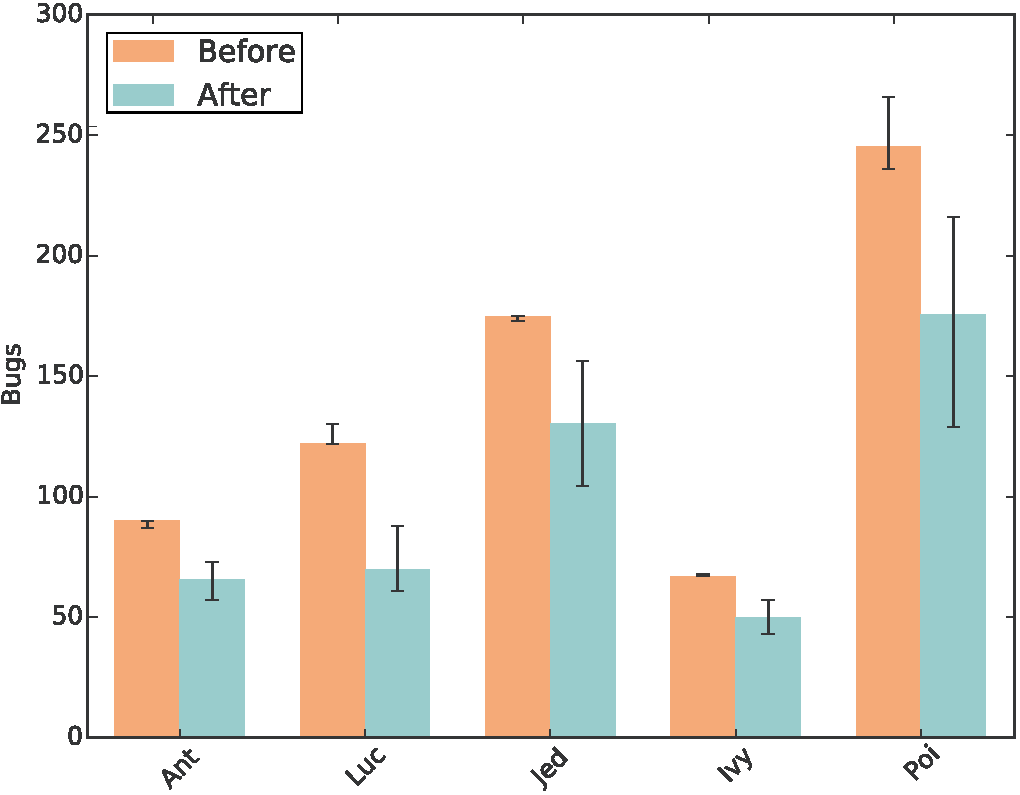
\includegraphics[width=\linewidth]{_figs/histograms.pdf}
\caption{Comparison of defects before and after planning.}
\label{fig:bugs}
\end{figure}
With this in mind, it is easy to note that lower cliffs delta score translates to better the performance. 

 
The results are tabulated in figure \ref{tab:ant}. For the sake of completeness, we have introduced three basic configurations in HERE: 
\bi
\item \textit{Extent of Mutation:} Denotes the extent by which a test instant is \textit{mutated} towards the best cluster in the contour. It is a fraction that lies between 0 and 1. The baseline study requires no change be made, and thus extent of mutation is set to zero.
\item \textit{Feature Weighting:} The importance of feature weighting has already been discussed in section \ref{fwt}. It is a fraction that lies between 0 and 1, with 0 being the least important and 1 the most important feature. The extent of mutation is multiplied by this fraction to determine how much a specific feature changes by. Generally, we would like to make the largest change to the most crucial feature.
\item \textit{Information Pruning:} In addition to the weighting the features, we explored the possibility of mutating only the most important features. The feature weights are already known to us, we sort the features in descending order of their weights and mutate only the first X\%.
\ei
It is to be noted however that 


\begin{figure*}[htbp!]

\noindent\begin{minipage}{0.5\textwidth}
  {\scriptsize \textbf{Ant}\\}
  {\scriptsize  \begin{tabular}{{l@{~~~~}l@{}r@{~~~~}r@{~~~~}c}}
      \arrayrulecolor{darkgray}
      \rowcolor[gray]{.9} \textbf{Rank} & \textbf{Treatment} & \textbf{Median} & \textbf{IQR} & \\
  1 & 0.75 &    -0.63  &  0.08 & \quart{2}{7}{5}{144} \\
  1 & 0.75, weighting &    -0.6  &  0.2 & \quart{0}{16}{8}{144} \\
\hline  2 & 0.5, weighting &    -0.42  &  0.11 & \quart{17}{10}{23}{144} \\
  2 & 0.5 &    -0.42  &  0.11 & \quart{19}{9}{23}{144} \\
  2 & 0.75, weighting, Prune=50\% &    -0.4  &  0.11 & \quart{20}{9}{25}{144} \\
\hline  3 & 0.25 &    -0.28  &  0.09 & \quart{31}{7}{35}{144} \\
  3 & 0.25, weighting &    -0.28  &  0.08 & \quart{31}{7}{35}{144} \\
\hline  4 & 0.5, weighting, Prune=50\% &    -0.25  &  0.06 & \quart{35}{5}{38}{144} \\
\hline  5 & 0.25, weighting, Prune=50\% &    -0.19  &  0.05 & \quart{41}{4}{43}{144} \\
\hline  6 & Baseline &    -0.11  &  0.03 & \quart{47}{2}{49}{144} \\
\hline \end{tabular}}
\end{minipage}
\noindent\begin{minipage}{0.5\textwidth}
  \flushleft
  {\scriptsize \textbf{Camel}\\}
{\scriptsize  \begin{tabular}{{l@{~~~~}l@{}r@{~~~~}r@{~~~~}c}}
\arrayrulecolor{darkgray}
\rowcolor[gray]{.9} \textbf{Rank} & \textbf{Treatment} & \textbf{Median} & \textbf{IQR} & \\
  1 &  0.75, weighting, Prune=50\% &    -0.41  &  0.1 & \quart{2}{14}{9}{205} \\
  1 &  0.75 &    -0.41  &  0.23 & \quart{1}{32}{9}{205} \\
  1 &  0.75, weighting &    -0.39  &  0.16 & \quart{0}{22}{12}{205} \\
\hline  2 &  0.5, weighting, Prune=50\% &    -0.27  &  0.09 & \quart{19}{12}{29}{205} \\
  2 &  0.5 &    -0.26  &  0.12 & \quart{20}{17}{30}{205} \\
  2 &  0.5, weighting &    -0.24  &  0.09 & \quart{24}{13}{33}{205} \\
\hline  3 &  0.25, weighting, Prune=50\% &    -0.2  &  0.05 & \quart{36}{7}{38}{205} \\
  3 &  0.25, weighting &    -0.19  &  0.07 & \quart{36}{9}{40}{205} \\
  3 &  0.25 &    -0.17  &  0.06 & \quart{37}{8}{43}{205} \\
\hline  4 &  Baseline &    -0.15  &  0.06 & \quart{41}{8}{45}{205} \\
\hline \end{tabular}}
\end{minipage}

\noindent\begin{minipage}{0.5\textwidth}
  \flushleft
  {\scriptsize \textbf{Ivy}\\[-0.05cm]}
{\scriptsize  \begin{tabular}{{l@{~~~~}l@{}r@{~~~~}r@{~~~~}c}}
\arrayrulecolor{darkgray}
\rowcolor[gray]{.9} \textbf{Rank} & \textbf{Treatment} & \textbf{Median} & \textbf{IQR} & \\
  1 &     0.75 &    -0.57  &  0.17 & \quart{0}{16}{6}{163} \\
  1 &   0.75, weighting &    -0.55  &  0.11 & \quart{3}{11}{8}{163} \\
\hline  2 &   0.75, weighting, Prune=50\% &    -0.38  &  0.11 & \quart{19}{11}{25}{163} \\
  2 &    0.5, weighting &    -0.36  &  0.12 & \quart{23}{12}{27}{163} \\
  2 &   0.5 &    -0.33  &  0.11 & \quart{25}{11}{30}{163} \\
\hline  3 &   0.5, weighting, Prune=50\% &    -0.27  &  0.08 & \quart{30}{8}{36}{163} \\
\hline  4 &   0.25, weighting &    -0.2  &  0.07 & \quart{41}{7}{43}{163} \\
  4 &     0.25 &    -0.16  &  0.04 & \quart{43}{4}{47}{163} \\
  4 &     Baseline &    -0.16  &  0.0 & \quart{47}{0}{47}{163} \\
\hline  5 &   0.25, weighting, Prune=50\% &    -0.15  &  0.04 & \quart{45}{4}{48}{163} \\
\hline \end{tabular}}
\end{minipage}
\noindent\begin{minipage}{0.5\textwidth}
  \flushleft
  {\scriptsize \textbf{Jedit}\\}
  {\scriptsize  \begin{tabular}{{l@{~~~~}l@{}r@{~~~~}r@{~~~~}c}}
\arrayrulecolor{darkgray}
\rowcolor[gray]{.9} \textbf{Rank} & \textbf{Treatment} & \textbf{Median} & \textbf{IQR} & \\
  1 &  0.75, weighting, Prune=50\% &    -0.41  &  0.18 & \quart{0}{20}{8}{172} \\
  1 &  0.75 &    -0.35  &  0.26 & \quart{0}{30}{15}{172} \\
\hline  2 &  0.75, weighting &    -0.25  &  0.17 & \quart{16}{20}{26}{172} \\
  2 &  0.5, weighting, Prune=50\% &    -0.21  &  0.1 & \quart{23}{11}{31}{172} \\
\hline  3 &   0.5 &    -0.17  &  0.08 & \quart{32}{9}{36}{172} \\
  3 &  0.5, weighting &    -0.14  &  0.09 & \quart{31}{10}{39}{172} \\
\hline  4 &  0.25, weighting, Prune=50\% &    -0.12  &  0.06 & \quart{39}{7}{41}{172} \\
\hline  5 &  0.25 &    -0.08  &  0.05 & \quart{43}{5}{46}{172} \\
  5 &  0.25, weighting &    -0.08  &  0.06 & \quart{43}{6}{46}{172} \\
\hline  6 &  Baseline &    -0.06  &  0.01 & \quart{47}{1}{48}{172} \\
\hline \end{tabular}}
\end{minipage}


\noindent\begin{minipage}{0.5\textwidth}
  \flushleft
  {\scriptsize \textbf{Log4j}\\}
  {\scriptsize  \begin{tabular}{{l@{~~~~}l@{}r@{~~~~}r@{~~~~}c}}
\arrayrulecolor{darkgray}
\rowcolor[gray]{.9} \textbf{Rank} & \textbf{Treatment} & \textbf{Median} & \textbf{IQR} & \\
  1 &  0.75, weighting, Prune=50\% &    -0.19  &  0.13 & \quart{0}{28}{15}{273} \\
\hline  2 &  0.75 &    -0.13  &  0.06 & \quart{23}{13}{28}{273} \\
  2 &  0.5, weighting, Prune=50\% &    -0.13  &  0.05 & \quart{23}{11}{28}{273} \\
  2 &  0.75, weighting &    -0.12  &  0.1 & \quart{15}{21}{30}{273} \\
\hline  3 &  0.5, weighting &    -0.1  &  0.03 & \quart{28}{6}{34}{273} \\
\hline  4 &   0.5 &    -0.1  &  0.07 & \quart{28}{15}{34}{273} \\
  4 &  0.25 &    -0.09  &  0.04 & \quart{34}{9}{36}{273} \\
  4 &  0.25, weighting, Prune=50\% &    -0.09  &  0.04 & \quart{34}{9}{36}{273} \\
  4 &  0.25, weighting &    -0.06  &  0.04 & \quart{34}{9}{43}{273} \\
\hline  5 &  Baseline &    -0.06  &  0.03 & \quart{43}{6}{43}{273} \\
\hline \end{tabular}}
\end{minipage}
\noindent\begin{minipage}{0.5\textwidth}
  \flushleft
  {\scriptsize \textbf{Lucene}\\}
  {\scriptsize  \begin{tabular}{{l@{~~~~}l@{}r@{~~~~}r@{~~~~}c}}
\arrayrulecolor{darkgray}
\rowcolor[gray]{.9} \textbf{Rank} & \textbf{Treatment} & \textbf{Median} & \textbf{IQR} & \\
  1 &  0.75, weighting &    -0.15  &  0.09 & \quart{0}{29}{9}{393} \\
  1 &  0.75 &    -0.13  &  0.09 & \quart{0}{29}{16}{393} \\
  1 &  0.75, weighting, Prune=50\% &    -0.12  &  0.08 & \quart{6}{27}{19}{393} \\
\hline  2 &  Baseline &    -0.1  &  0.03 & \quart{26}{10}{26}{393} \\
  2 &  0.5, weighting, Prune=50\% &    -0.1  &  0.03 & \quart{23}{10}{26}{393} \\
\hline  3 &  0.5, weighting &    -0.08  &  0.06 & \quart{23}{20}{33}{393} \\
  3 &  0.25, weighting, Prune=50\% &    -0.07  &  0.03 & \quart{33}{10}{36}{393} \\
  3 &  0.5 &    -0.07  &  0.05 & \quart{29}{17}{36}{393} \\
\hline  4 &  0.25, weighting &    -0.04  &  0.04 & \quart{36}{13}{46}{393} \\
  4 &  0.25 &    -0.04  &  0.02 & \quart{39}{7}{46}{393} \\
\hline \end{tabular}}
\end{minipage}

\noindent\begin{minipage}{0.5\textwidth}
  \flushleft
  {\scriptsize \textbf{Poi}\\}
  {\scriptsize  \begin{tabular}{{l@{~~~~}l@{}r@{~~~~}r@{~~~~}c}}
      \arrayrulecolor{darkgray}
\rowcolor[gray]{.9} \textbf{Rank} & \textbf{Treatment} & \textbf{Median} & \textbf{IQR} & \\
  1 & 0.75, weighting &    -0.45  &  0.1 & \quart{6}{10}{11}{162} \\
  1 &  0.75 &    -0.44  &  0.23 & \quart{0}{23}{12}{162} \\
\hline  2 & 0.5, weighting &    -0.32  &  0.23 & \quart{12}{24}{24}{162} \\
  2 & 0.5 &    -0.26  &  0.23 & \quart{18}{24}{31}{162} \\
  2 & 0.75, weighting, Prune=50\% &    -0.25  &  0.19 & \quart{17}{20}{32}{162} \\
\hline  3 & 0.5, weighting, Prune=50\% &    -0.19  &  0.09 & \quart{34}{9}{38}{162} \\
  3 &  0.25 &    -0.19  &  0.11 & \quart{32}{11}{38}{162} \\
  3 & 0.25, weighting &    -0.17  &  0.14 & \quart{30}{14}{40}{162} \\
\hline  4 & 0.25, weighting, Prune=50\% &    -0.12  &  0.09 & \quart{40}{9}{45}{162} \\
\hline  5 &  Baseline &    -0.09  &  0.03 & \quart{46}{3}{48}{162} \\
\hline \end{tabular}}
\end{minipage}
\noindent\begin{minipage}{0.5\textwidth}
  \flushleft
  {\scriptsize \textbf{Synapse}\\}
  {\scriptsize  \begin{tabular}{{l@{~~~~}l@{}r@{~~~~}r@{~~~~}c}}
\arrayrulecolor{darkgray}
\rowcolor[gray]{.9} \textbf{Rank} & \textbf{Treatment} & \textbf{Median} & \textbf{IQR} & \\
  1 & 0.75, weighting &    -0.56  &  0.2 & \quart{7}{18}{11}{148} \\
  1 & 0.75 &    -0.48  &  0.34 & \quart{0}{29}{18}{148} \\
\hline  2 & 0.5 &    -0.4  &  0.27 & \quart{14}{24}{25}{148} \\
  2 & 0.5, weighting &    -0.37  &  0.17 & \quart{21}{15}{28}{148} \\
\hline  3 & 0.25 &    -0.23  &  0.16 & \quart{31}{14}{40}{148} \\
  3 & 0.25, weighting &    -0.23  &  0.1 & \quart{38}{9}{40}{148} \\
  3 & 0.75, weighting, Prune=50\% &    -0.19  &  0.08 & \quart{40}{7}{43}{148} \\
\hline  4 & 0.25, weighting, Prune=50\% &    -0.17  &  0.08 & \quart{42}{7}{45}{148} \\
  4 & Baseline &    -0.15  &  0.0 & \quart{47}{0}{47}{148} \\
  4 & 0.5, weighting, Prune=50\% &    -0.15  &  0.11 & \quart{40}{9}{47}{148} \\
\hline \end{tabular}}
\end{minipage}

\noindent\begin{minipage}{0.50\textwidth}
  \flushleft
  {\scriptsize \textbf{Velocity}\\}
  {\scriptsize  \begin{tabular}{{l@{~~~~}l@{}r@{~~~~}r@{~~~~}c}}
\arrayrulecolor{darkgray}
\rowcolor[gray]{.9} \textbf{Rank} & \textbf{Treatment} & \textbf{Median} & \textbf{IQR} & \\
  1 & 0.75, weighting &    -0.19  &  0.22 & \quart{1}{34}{21}{207} \\
  1 & 0.75, weighting, Prune=50\% &    -0.15  &  0.13 & \quart{14}{20}{28}{207} \\
  1 & 0.75 &    -0.14  &  0.23 & \quart{0}{35}{29}{207} \\
\hline  2 & 0.5 &    -0.13  &  0.11 & \quart{23}{17}{31}{207} \\
\hline  3 & 0.5, weighting &    -0.1  &  0.08 & \quart{29}{13}{35}{207} \\
  3 & 0.5, weighting, Prune=50\% &    -0.07  &  0.07 & \quart{32}{11}{40}{207} \\
\hline  4 & Baseline &    -0.05  &  0.04 & \quart{43}{6}{43}{207} \\
  4 & 0.25, weighting &    -0.05  &  0.03 & \quart{40}{5}{43}{207} \\
  4 & 0.25 &    -0.04  &  0.02 & \quart{43}{3}{45}{207} \\
  4 & 0.25, weighting, Prune=50\% &    -0.01  &  0.04 & \quart{43}{6}{49}{207} \\
\hline \end{tabular}}
\end{minipage}
\noindent\begin{minipage}{0.50\textwidth}
  \flushleft
  {\scriptsize \textbf{Xalan}\\}
  {\scriptsize  \begin{tabular}{{l@{~~~~}l@{}r@{~~~~}r@{~~~~}c}}
\arrayrulecolor{darkgray}
\rowcolor[gray]{.9} \textbf{Rank} & \textbf{Treatment} & \textbf{Median} & \textbf{IQR} & \\
  1 & 0.75 &    -0.36  &  0.12 & \quart{0}{16}{9}{198} \\
  1 & 0.75, weighting &    -0.3  &  0.17 & \quart{4}{23}{18}{198} \\
  1 &    0.5 &    -0.3  &  0.12 & \quart{9}{17}{18}{198} \\
\hline  2 & 0.5, weighting &    -0.28  &  0.09 & \quart{16}{13}{20}{198} \\
\hline  3 & 0.25, weighting &    -0.23  &  0.1 & \quart{20}{14}{27}{198} \\
  3 & 0.25 &    -0.23  &  0.12 & \quart{20}{17}{27}{198} \\
\hline  4 & 0.25, weighting, Prune=50\% &    -0.14  &  0.07 & \quart{36}{9}{40}{198} \\
  4 & 0.75, weighting, Prune=50\% &    -0.14  &  0.07 & \quart{33}{10}{40}{198} \\
  4 & 0.5, weighting, Prune=50\% &    -0.12  &  0.06 & \quart{37}{8}{43}{198} \\
\hline  5 & Baseline &    -0.08  &  0.02 & \quart{47}{2}{48}{198} \\
\hline \end{tabular}}
\end{minipage}
\caption{Cliffs Delta Scores for the defect data set. The Treatment column, has 3 possible configurations, the first (0.25, 0.50, and 0.75) represents the extent of mutation; weighting represents feature weighting; Prune represents the extent of information pruning.}
\label{tab:ant}
\end{figure*}



\begin{figure*}[htbp!]
\centering
\begin{minipage}{0.30\linewidth}
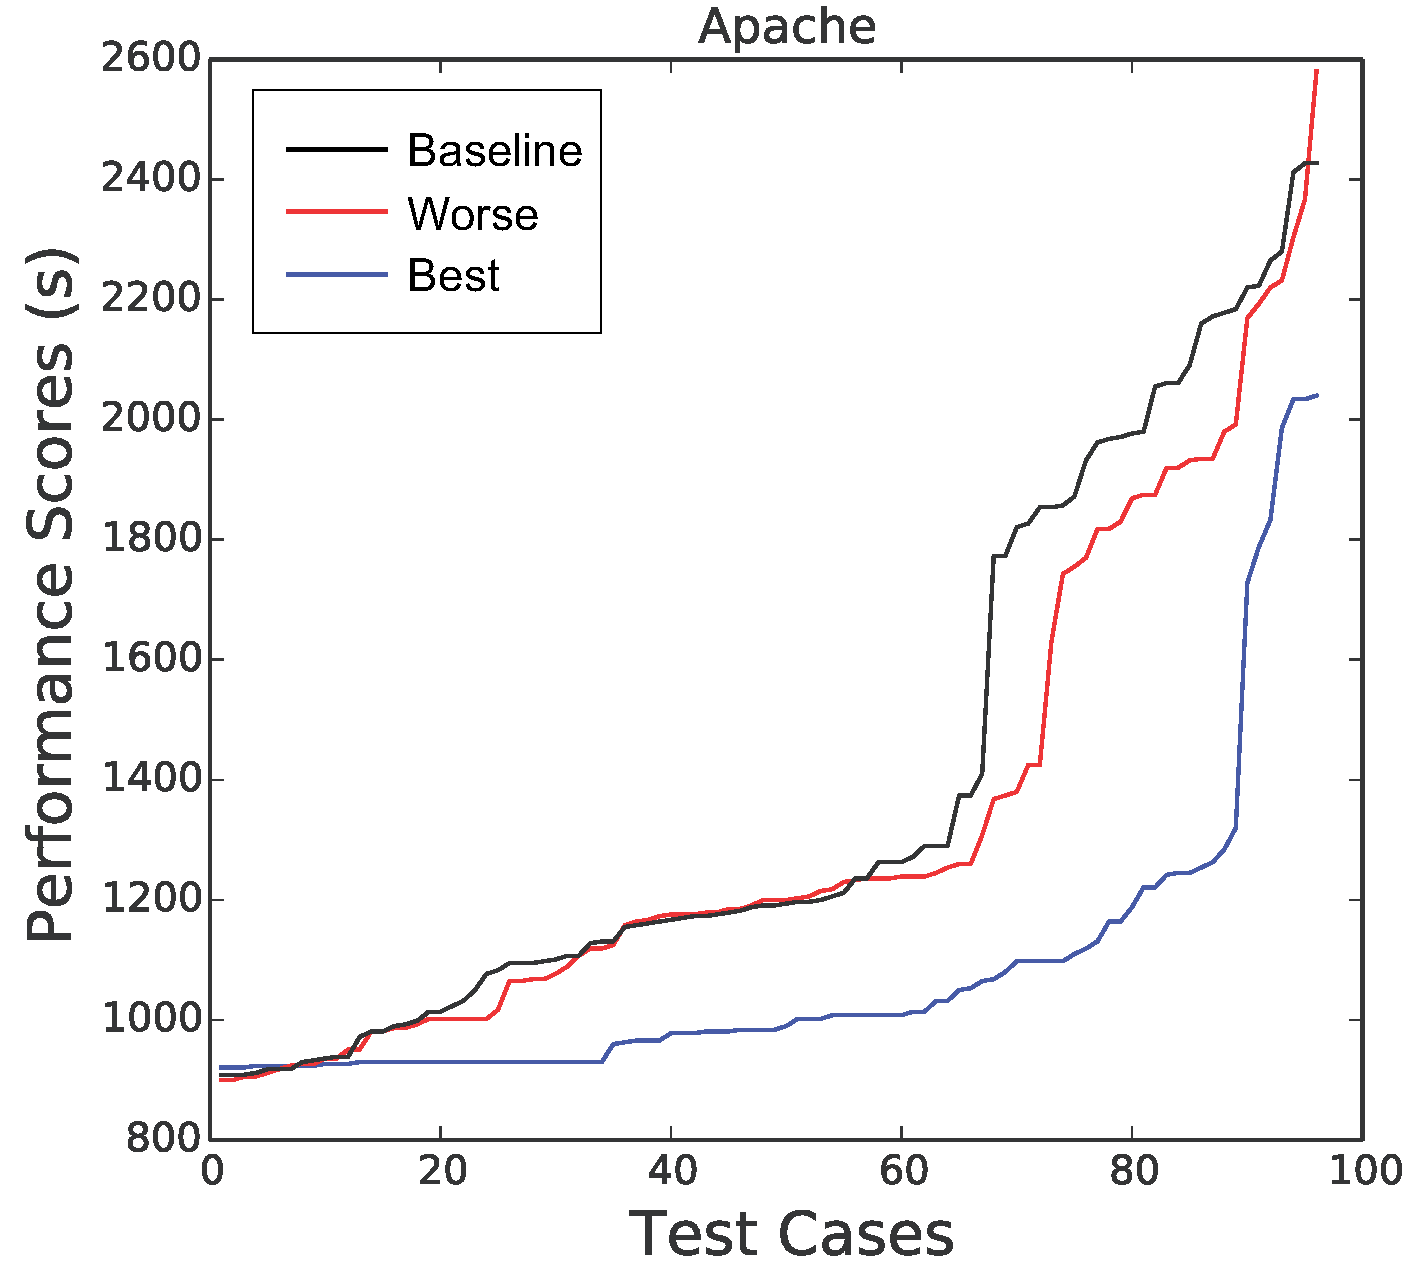
\includegraphics[width=\linewidth]{_figs/Apache.pdf}
\end{minipage}
\begin{minipage}{0.30\linewidth}
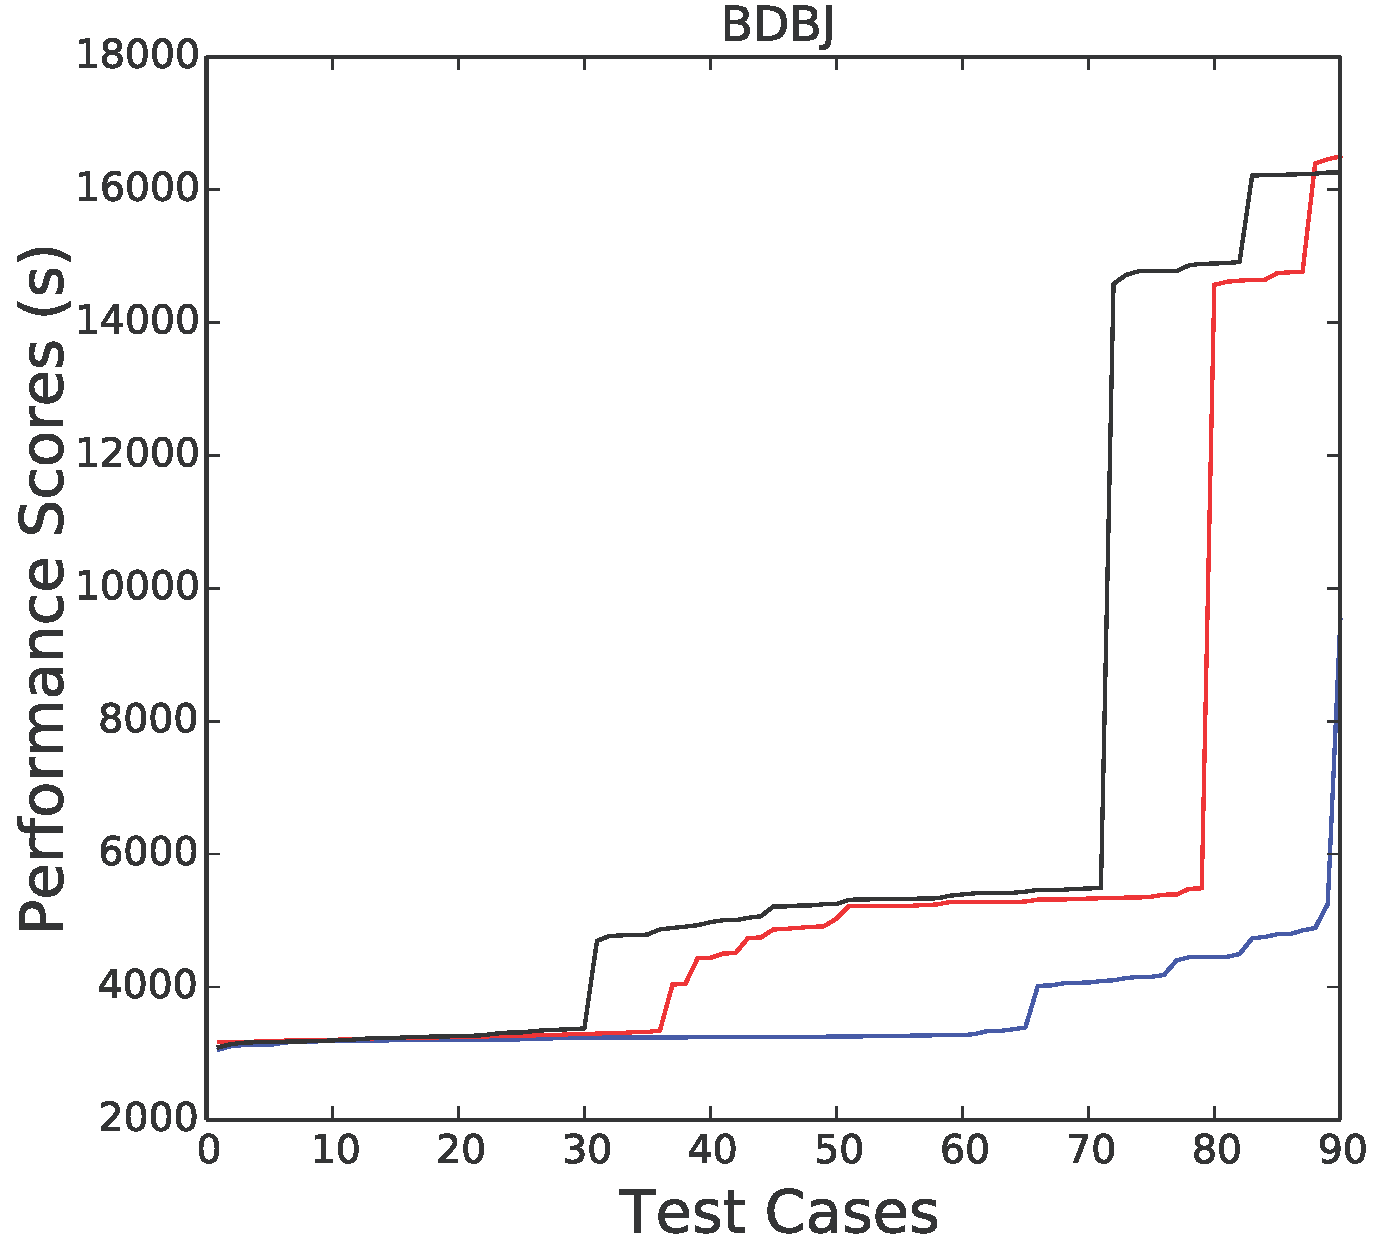
\includegraphics[width=\linewidth]{_figs/BDBJ.pdf}
\end{minipage}
\begin{minipage}{0.30\linewidth}
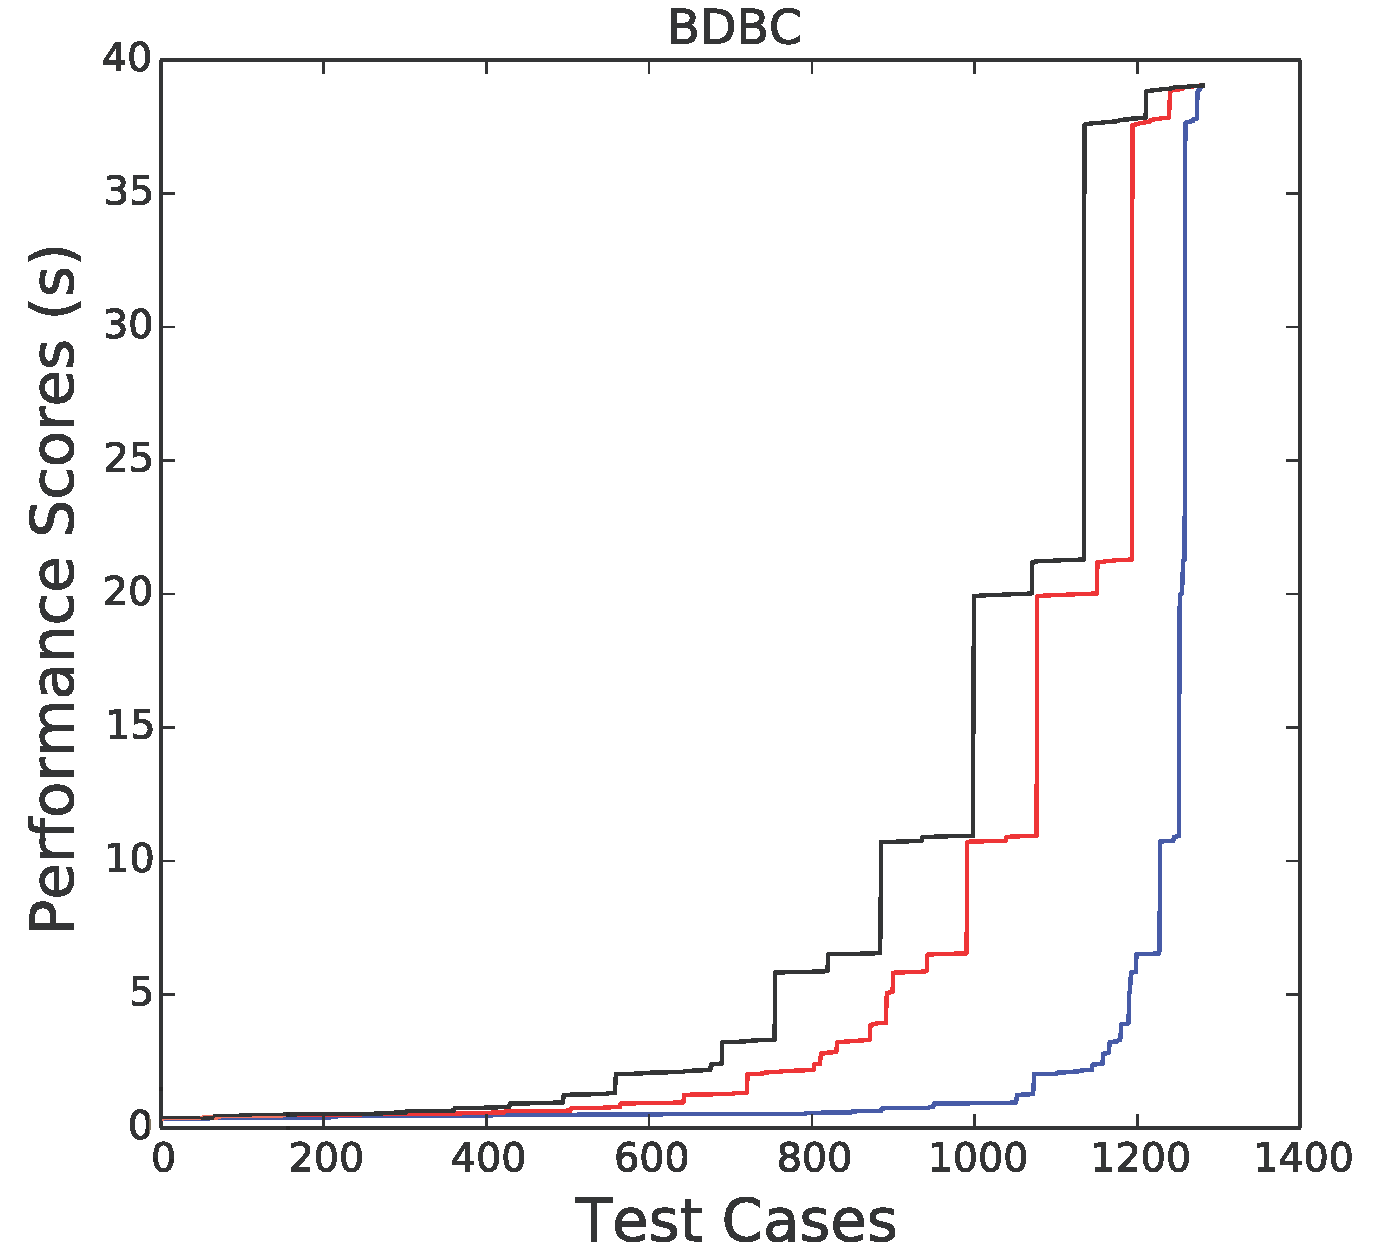
\includegraphics[width=\linewidth]{_figs/BDBC.pdf}
\end{minipage}

\begin{minipage}{0.30\linewidth}
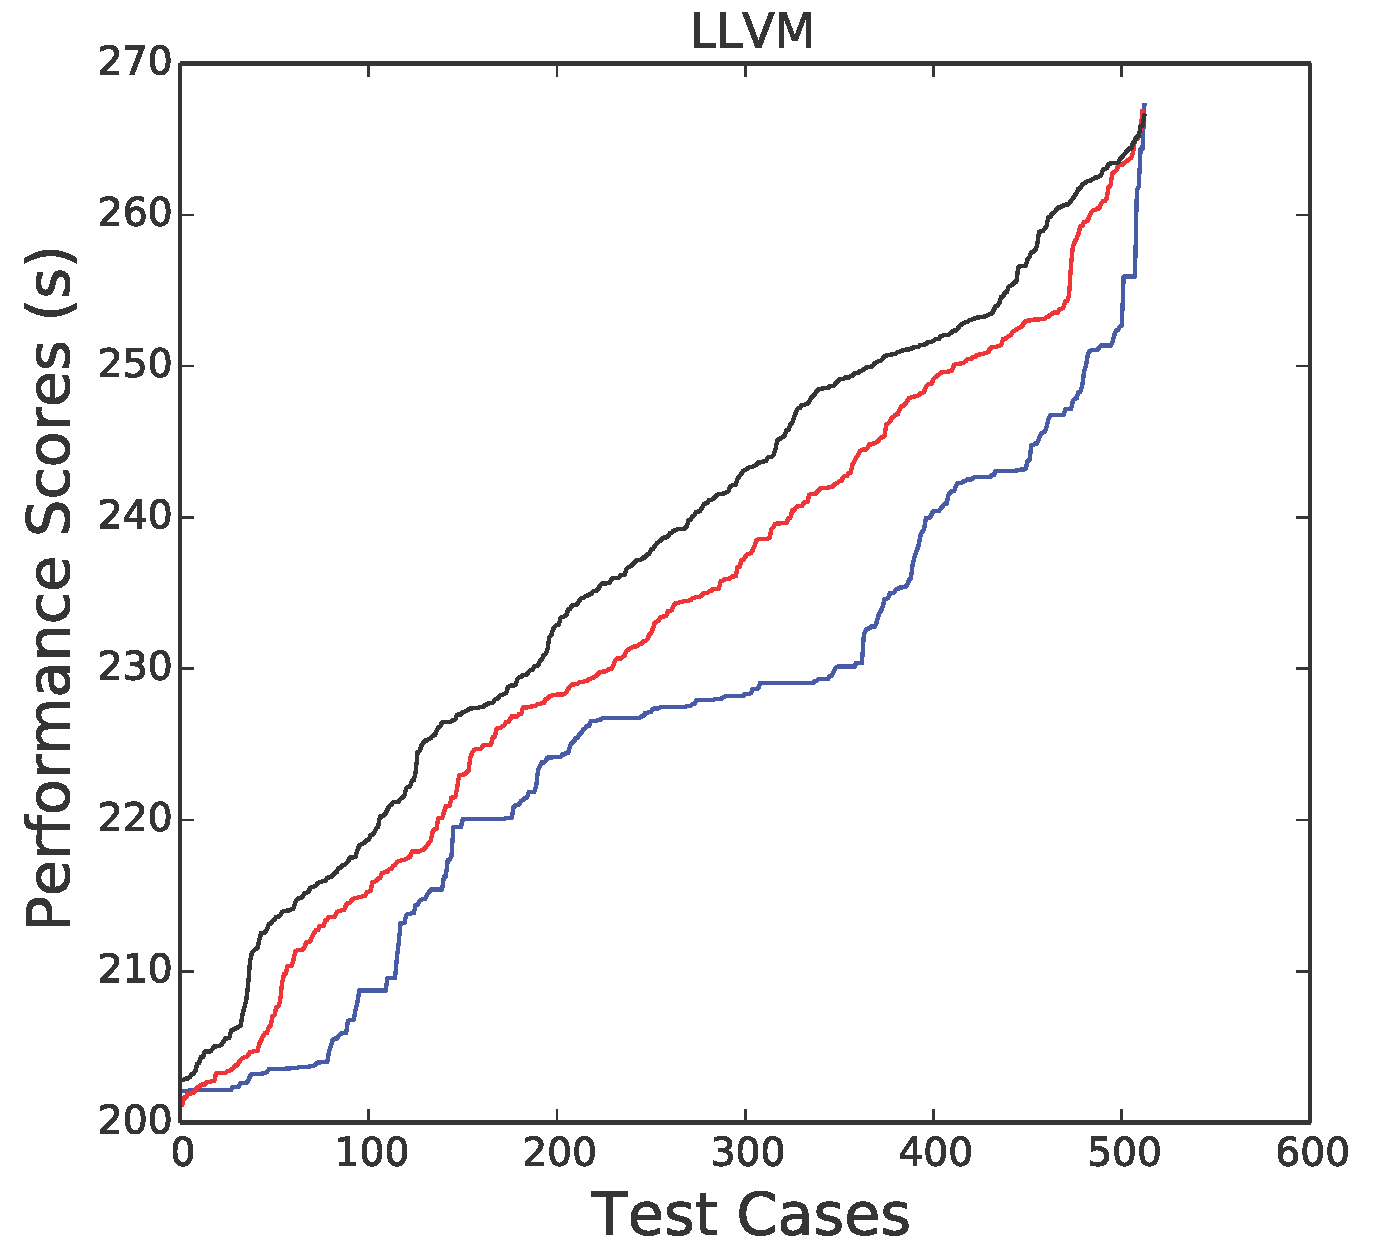
\includegraphics[width=\linewidth]{_figs/LLVM.pdf}
\end{minipage}
\begin{minipage}{0.30\linewidth}
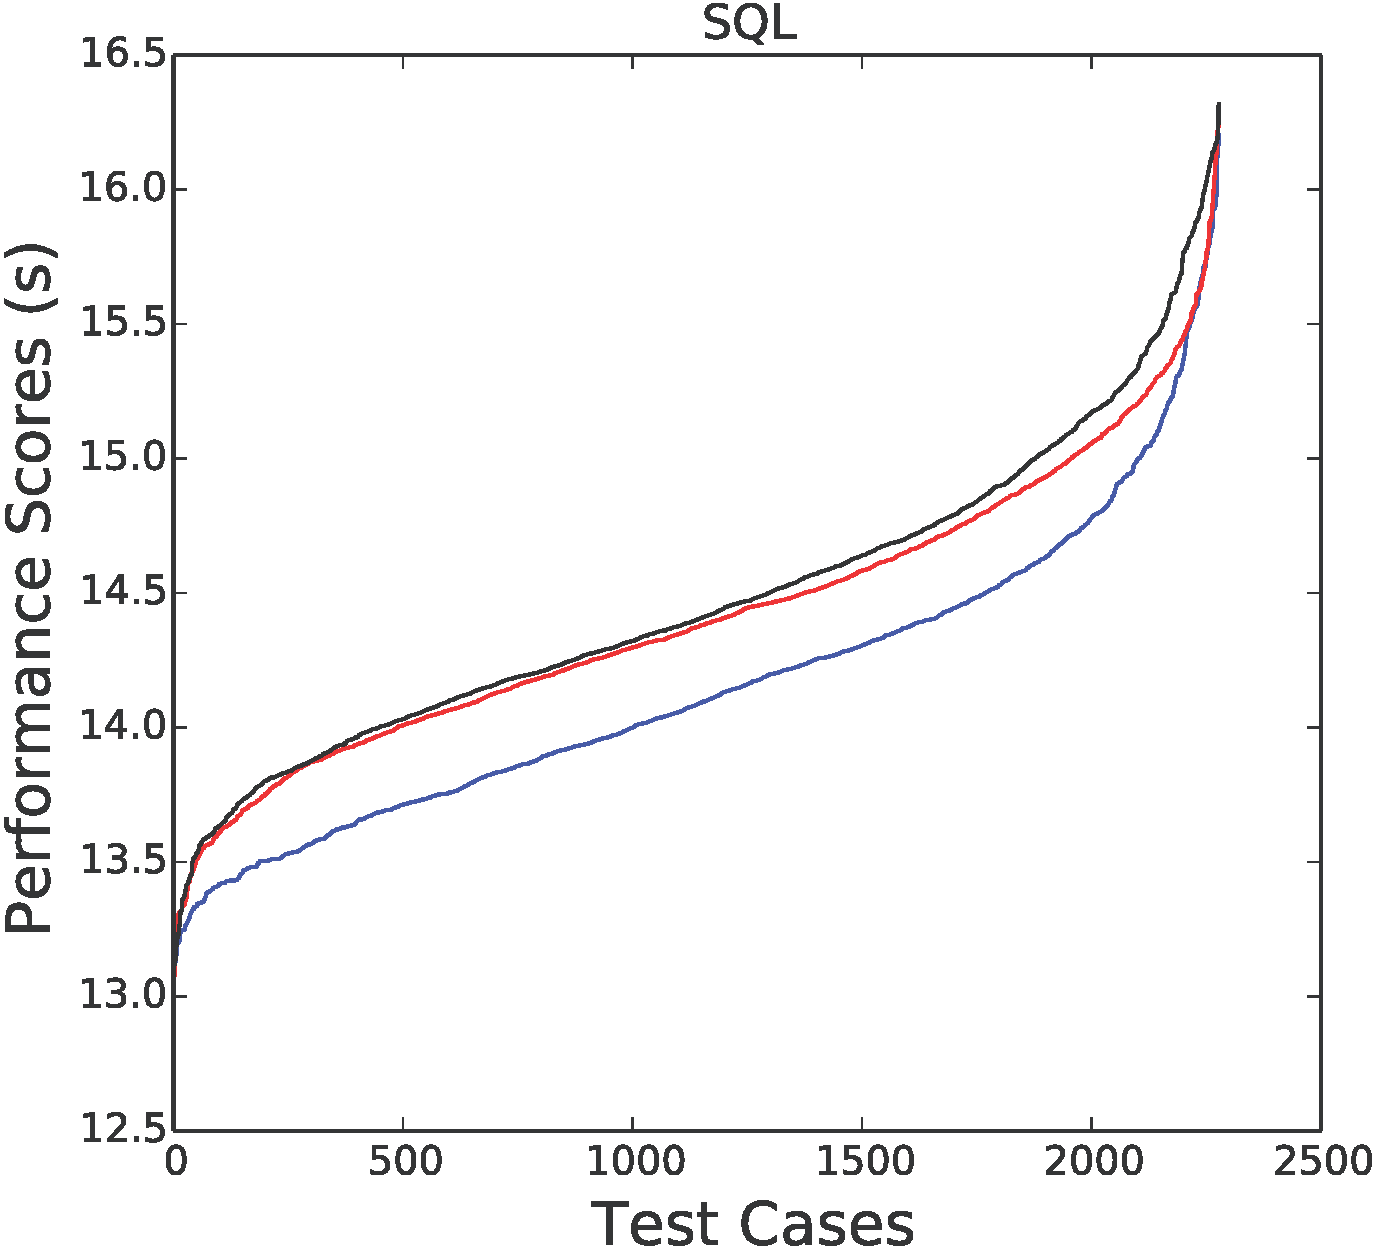
\includegraphics[width=\linewidth]{_figs/SQL.pdf}
\end{minipage}
\begin{minipage}{0.30\linewidth}
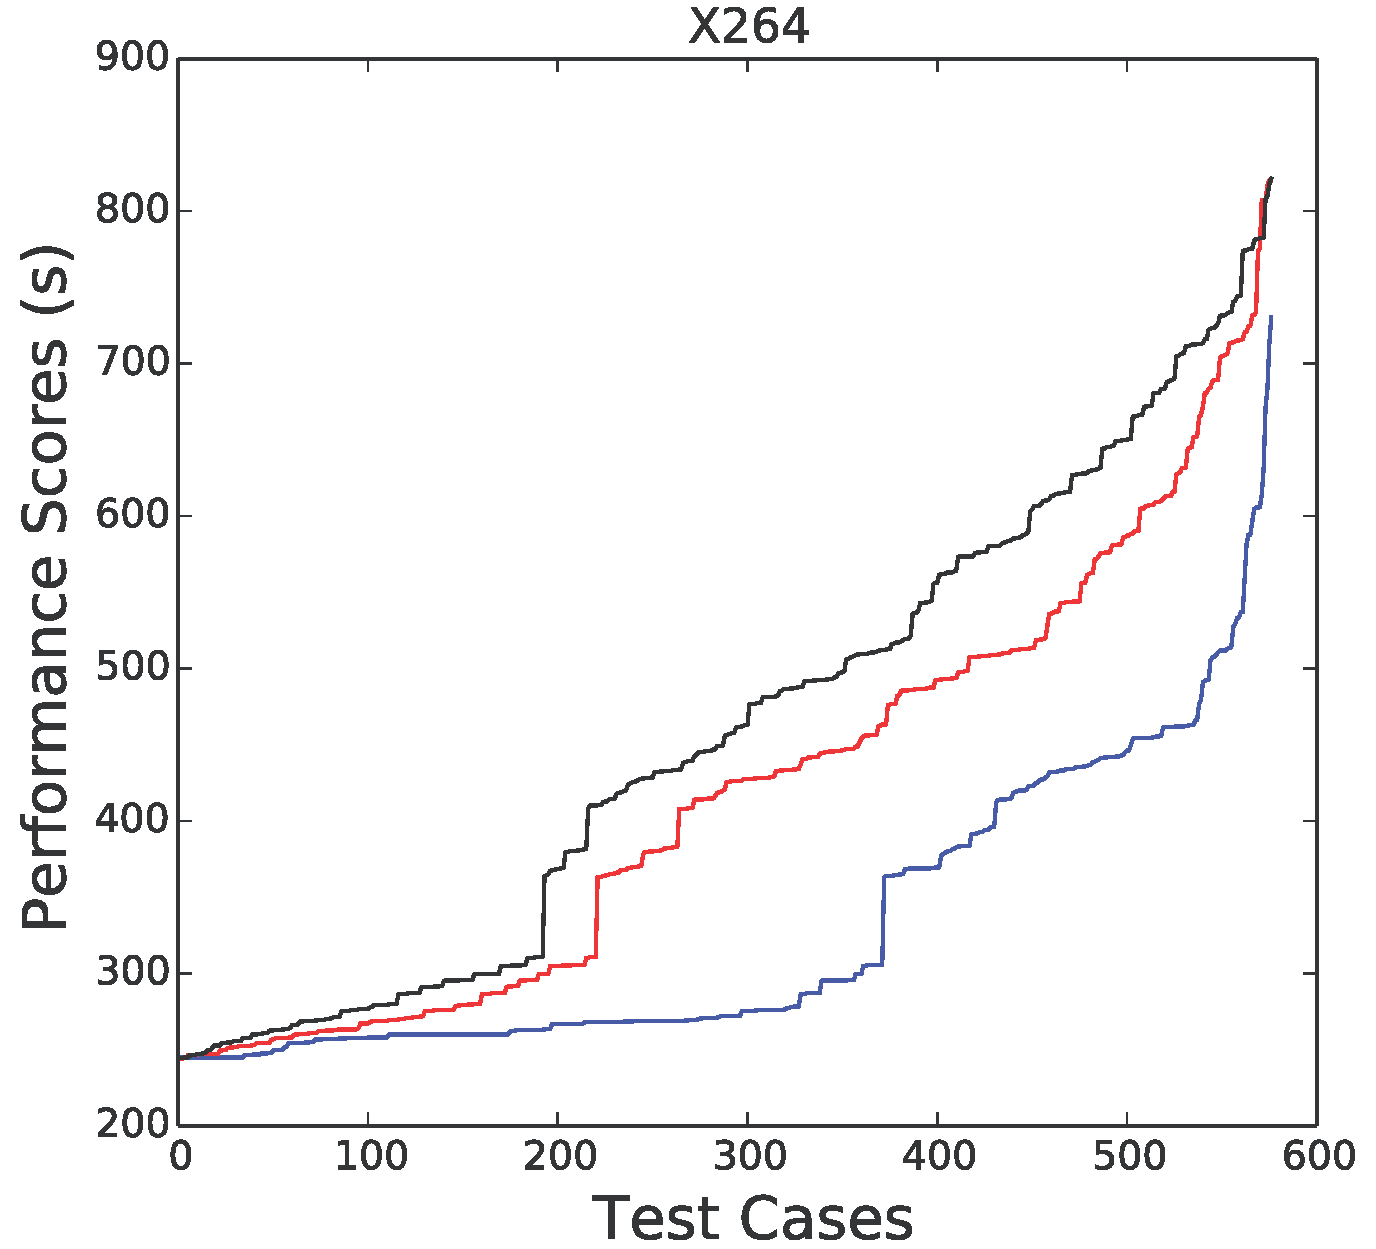
\includegraphics[width=\linewidth]{_figs/X264.pdf}
\end{minipage}
\caption{Run time optimization using HERE. Blue curve represents a mutation probability of 0.75 with feature weighting and information pruning; Red curve represents a mutation probability of 0.25 with feature weighting, but no information pruning; Black curve represents the raw test data used as baseline for the comparison.}
\label{fig:pp}
\end{figure*}


\subsection{Performance Prediction Data set}

In this section, 
\begin{figure*}[htbp!]
\noindent\begin{minipage}{0.5\textwidth}
  {\scriptsize \textbf{Apache}\\}
  {\scriptsize  \begin{tabular}{{l@{~~~~}l@{~~~~}r@{~~~~}r@{~~~~}c}}
      \arrayrulecolor{darkgray}
      \rowcolor[gray]{.9} \textbf{Rank} & \textbf{Treatment} & \textbf{Median} & \textbf{IQR} & \\
  1 & 75, weighting, Prune=25\% &    0.77  &  0.05 & \quart{0}{9}{3}{49} \\
  1 &   75 &    0.79  &  0.08 & \quart{1}{16}{7}{49} \\
\hline  2 & 75, weighting &    0.85  &  0.07 & \quart{9}{14}{19}{49} \\
  2 & 50, weighting, Prune=25\% &    0.85  &  0.04 & \quart{15}{8}{19}{49} \\
  2 &  50 &    0.85  &  0.05 & \quart{17}{10}{19}{49} \\
\hline  3 & 50, weighting &    0.91  &  0.05 & \quart{25}{10}{31}{49} \\
  3 &  25 &    0.92  &  0.04 & \quart{29}{8}{33}{49} \\
  3 & 25, weighting, Prune=25\% &    0.93  &  0.02 & \quart{33}{4}{35}{49} \\
\hline  4 & 25, weighting &    0.96  &  0.03 & \quart{37}{6}{41}{49} \\
\hline  5 & baseline &    1.0  &  0.0 & \quart{49}{0}{49}{49} \\
\hline \end{tabular}}
\end{minipage}
\noindent\begin{minipage}{0.5\textwidth}
  \flushleft
  {\scriptsize \textbf{BDBC}\\}
{\scriptsize  \begin{tabular}{{l@{~~~~}l@{~~~~}r@{~~~~}r@{~~~~}c}}
\arrayrulecolor{darkgray}
\rowcolor[gray]{.9} \textbf{Rank} & \textbf{Treatment} & \textbf{Median} & \textbf{IQR} & \\
  1 &     75 &    0.22  &  0.05 & \quart{0}{3}{1}{49} \\
  1 &  75, weighting, Prune=25\% &    0.21  &  0.04 & \quart{0}{2}{0}{49} \\
\hline  2 &  75, weighting &    0.24  &  0.1 & \quart{0}{6}{2}{49} \\
\hline  3 &     50 &    0.4  &  0.04 & \quart{11}{2}{12}{49} \\
  3 &  50, weighting, Prune=25\% &    0.4  &  0.05 & \quart{10}{3}{12}{49} \\
\hline  4 &  50, weighting &    0.47  &  0.09 & \quart{14}{5}{16}{49} \\
\hline  5 &     25 &    0.66  &  0.03 & \quart{28}{1}{28}{49} \\
  5 &  25, weighting, Prune=25\% &    0.67  &  0.06 & \quart{28}{3}{29}{49} \\
\hline  6 &  25, weighting &    0.69  &  0.06 & \quart{29}{4}{30}{49} \\
\hline  7 &  baseline &    1.0  &  0.0 & \quart{49}{0}{49}{49} \\
\hline \end{tabular}}
\end{minipage}

\noindent\begin{minipage}{0.5\textwidth}
  \flushleft
  {\scriptsize \textbf{BDBJ}\\}
{\scriptsize  \begin{tabular}{{l@{~~~~}l@{~~~~}r@{~~~~}r@{~~~~}c}}
\arrayrulecolor{darkgray}
\rowcolor[gray]{.9} \textbf{Rank} & \textbf{Treatment} & \textbf{Median} & \textbf{IQR} & \\
  1 &     75 &    0.63  &  0.16 & \quart{0}{19}{3}{49} \\
  1 &  75, weighting, Prune=25\% &    0.68  &  0.17 & \quart{1}{21}{9}{49} \\
  1 &  75, weighting &    0.74  &  0.11 & \quart{8}{14}{17}{49} \\
\hline  2 &  50, weighting, Prune=25\% &    0.75  &  0.09 & \quart{14}{12}{18}{49} \\
  2 &     50 &    0.79  &  0.13 & \quart{16}{16}{23}{49} \\
\hline  3 &  50, weighting &    0.82  &  0.09 & \quart{23}{11}{27}{49} \\
\hline  4 &  25, weighting, Prune=25\% &    0.87  &  0.07 & \quart{29}{9}{33}{49} \\
\hline  5 &     25 &    0.88  &  0.06 & \quart{33}{8}{34}{49} \\
  5 &  25, weighting &    0.92  &  0.06 & \quart{36}{7}{39}{49} \\
\hline  6 &  baseline &    1.0  &  0.0 & \quart{49}{0}{49}{49} \\
\hline \end{tabular}}
\end{minipage}
\noindent\begin{minipage}{0.5\textwidth}
  \flushleft
  {\scriptsize \textbf{LLVM}\\}
  {\scriptsize  \begin{tabular}{{l@{~~~~}l@{~~~~}r@{~~~~}r@{~~~~}c}}
\arrayrulecolor{darkgray}
\rowcolor[gray]{.9} \textbf{Rank} & \textbf{Treatment} & \textbf{Median} & \textbf{IQR} & \\
  1 &     75 &    0.92  &  0.01 & \quart{5}{6}{5}{49} \\
  1 &  75, weighting, Prune=25\% &    0.92  &  0.02 & \quart{0}{11}{5}{49} \\
  1 &  75, weighting &    0.93  &  0.02 & \quart{5}{11}{11}{49} \\
\hline  2 &     50 &    0.94  &  0.01 & \quart{16}{6}{16}{49} \\
  2 &  50, weighting, Prune=25\% &    0.95  &  0.0 & \quart{22}{0}{22}{49} \\
  2 &  50, weighting &    0.96  &  0.02 & \quart{22}{11}{27}{49} \\
\hline  3 &     25 &    0.98  &  0.01 & \quart{33}{5}{38}{49} \\
  3 &  25, weighting, Prune=25\% &    0.98  &  0.01 & \quart{33}{5}{38}{49} \\
  3 &  25, weighting &    0.98  &  0.0 & \quart{38}{0}{38}{49} \\
\hline  4 &  baseline &    1.0  &  0.0 & \quart{49}{0}{49}{49} \\
\hline \end{tabular}}
\end{minipage}


\noindent\begin{minipage}{0.5\textwidth}
  \flushleft
  {\scriptsize \textbf{SQL}\\}
  {\scriptsize  \begin{tabular}{{l@{~~~~}l@{~~~~}r@{~~~~}r@{~~~~}c}}
\arrayrulecolor{darkgray}
\rowcolor[gray]{.9} \textbf{Rank} & \textbf{Treatment} & \textbf{Median} & \textbf{IQR} & \\
  1 &      75 &    0.98  &  0.01 & \quart{0}{16}{16}{49} \\
  1 &  75, weighting, Prune=25\% &    0.98  &  0.0 & \quart{16}{0}{16}{49} \\
  1 &  75, weighting &    0.99  &  0.01 & \quart{16}{17}{33}{49} \\
  1 &  50, weighting, Prune=25\% &    0.99  &  0.0 & \quart{33}{0}{33}{49} \\
  1 &      50 &    0.99  &  0.0 & \quart{33}{0}{33}{49} \\
  1 &  50, weighting &    0.99  &  0.01 & \quart{33}{16}{33}{49} \\
  1 &  25, weighting, Prune=25\% &    1.0  &  0.0 & \quart{49}{0}{49}{49} \\
  1 &      25 &    1.0  &  0.0 & \quart{49}{0}{49}{49} \\
  1 &  25, weighting &    1.0  &  0.0 & \quart{49}{0}{49}{49} \\
  1 &  baseline &    1.0  &  0.0 & \quart{49}{0}{49}{49} \\
  \hline \end{tabular}}
\end{minipage}
\noindent\begin{minipage}{0.5\textwidth}
  \flushleft
  {\scriptsize \textbf{X264}\\}
  {\scriptsize  \begin{tabular}{{l@{~~~~}l@{~~~~}r@{~~~~}r@{~~~~}c}}
\arrayrulecolor{darkgray}
\rowcolor[gray]{.9} \textbf{Rank} & \textbf{Treatment} & \textbf{Median} & \textbf{IQR} & \\
  1 &  75, weighting, Prune=25\% &    0.73  &  0.05 & \quart{1}{9}{3}{49} \\
  1 &     75 &    0.74  &  0.05 & \quart{0}{8}{5}{49} \\
\hline  2 &  75, weighting &    0.81  &  0.04 & \quart{13}{7}{17}{49} \\
  2 &  50, weighting, Prune=25\% &    0.82  &  0.04 & \quart{17}{7}{18}{49} \\
  2 &     50 &    0.83  &  0.03 & \quart{17}{5}{20}{49} \\
\hline  3 &  50, weighting &    0.88  &  0.03 & \quart{25}{6}{29}{49} \\
\hline  4 &     25 &    0.9  &  0.03 & \quart{31}{5}{32}{49} \\
  4 &  25, weighting, Prune=25\% &    0.91  &  0.03 & \quart{32}{5}{34}{49} \\
\hline  5 &  25, weighting &    0.93  &  0.02 & \quart{36}{3}{37}{49} \\
\hline  6 &  baseline &    1.0  &  0.0 & \quart{49}{0}{49}{49} \\
\hline \end{tabular}}
\end{minipage}
\end{figure*}


% \section{Discussion}
\section{Threats to validity}


\section{Related Work}
The connection of HOW to model-based evolutionary programming was discussed above.
In summary,   model-based tools such as NSGA-III~\cite{deb14} or MOEA/D~\cite{zhang07:TEC}
use some domain model as part of extensive Monte Carlo studies (augmented with some
evolution of selected best instances).
The premise of HOW is that we have access to domain data, but not a domain model.
Also, the results shown above were obtained without evolving/updating some current population
multiple times.


Planning with HERE is somewhat different to the recommendor systems.
As described by Robillard and Walker~\cite{rob14}, recommendor systems
in software engineering
are less {\em directive} and more    {\em collaborative} than policy
generators:
\bi
\item
Directive systems such as HERE tell developers exactly what to do
(e.g. ``use these settings in a Makefile'') 
\item
The collaborative systems discussed by Robillard and Walker
are more suggestive guides that
help (e.g.) programmers focus on very small sets
with  very large libraries of code of documentation.
\ei
One difference between directive and collaborative systems is that
the latter may not presume to suggest exactly what to do next.
However, planning systems like HOW are much more ardent: then make precise recommendations
of how to change all items in the test suite.
 

HOW is more a data mining method than a model-based optimizer. It represents our next attempt
to develop model-less instance-based optimizers.  Our previous attempts in this area
were the W2, WHERE, and IDEA systems~~\cite{menzies13:brady,Menzies2013:local,me12c}.
W2 was developed with Brady et al.~\cite{menzies13:brady}. 
W2 reasoned over deltas in the the raw
attributes values (and not the synthesized attributes used by HOW). 
The results of  adjusting values via those deltas was assessed via an SQL-like
query that selected all examples in the database that satisfied the newly adjusted
values. W2 suffers from two problems that are resolved
in this paper: {\em optimization failure} and {\em instance exhastion}.
\bi
\item 
As reported in that paper, W2
had a large number of {\em optimization failures}; i.e. after applying its recommendations,
the objective scores actually got worse. We recommend HOW's approach (of reasoning
over the synthesized attributes) to W2 since {\em in none of the above
results} do we observe that {\em after} we treat the data, that the objective scores are worse.
\item
As to {\em instance exhaustion}, W2 was a simple case-based reasoning system that never generalized
over its instances. Hence, the SQl-like query used to asses W2's plans often returned
a vanishingly small number of instances. To avoid this problem, we strongly recommend
combining a planning system with a prediction system (as done in this paper) such that we can
generalize to adjusted examples not seen on the original sample.
\ei
The WHERE tool~\cite{Menzies2013:local} developed the recursive clustering method over synthesized attributes
  used in this paper. WHERE was   a prediction
system since reported current patterns in the data, rather than proposing plans
on how to improve those patterns. Nor did that tool offer guidance on how to assess
the results of stepping along those patterns to guide changes to the system.

The problems of W2 and the success of WHERE suggested in might be useful to combine
WHERE's synthesized attributes with W2. The result was the IDEA tool~\cite{me12c}. 
While the initial prototype seemed promising~\cite{me12c}, we made the mistake of using
the tree structure of the recursive clusters to generate plans (in IDEA, the plan to
move an instance from one poorly performing cluster $C_1$ to another $C_2$ was computed
from the different in the  median
values of the instances in the two  branches that lead to $C_1$ and $C_2$).  When
that approach was applied to the data used in this paper, the results were quite weak
(very little net improvement). However, we abandoned the tree-query approach
and went for the pure instance-based approach discussed at the start of this paper.


Moving on to other releated work, depending on the audience  we would
 call HOW a {\em spectral learner}, 
a {\em response surface method}, or  a {\em local search operator}.
According to
Kamvar et al~\cite{kamvar03}
{\em spectral learners}reason across $m$ underlying dimensions synthesized
using (say) PCA~\cite{pearson1901}. For example,
algorithms like PDDP~\cite{boley98} use PCA to
recursively divide data into smaller regions where each level of recursion needs an   $O(N^2)$ analysis
to infer the principle components. HOW performs an analogous procedure using a   $O(2N)$ analysis
based on a heuristic proposed by
Faloutsos and Lin~\cite{Faloutsos1995} (see above, the ``FASTMAP'' algorithm).

{\em Response surface methods}  build a fast approximation to the function being optimized,
then uses that  approximation to take intelligent guesses about useful mutations. HOW
is a non-parametric response surface method that finds its response surface via recursive
clustering. For an example of a parametric response surface method, that uses Gaussian process
models, see Zuluaga et al.~\cite{zuluaga13}.

A {\em local search operator} that a some probability $p$, nudges  instance variables
along a dimension that improves its objective scores. HOW's recursive clustering methods
combine $n$ dimensions into $m \ll n$ so its ``nudges'' are simultaneous
adjustments along multiple dimensions. For an example of other kinds of local search algorithms, that only adjust
one variable at a time, see the literature on WALKSAT~\cite{Selman1992} and MAXWALKSAT~\cite{kautz97}.
See also the literature on local search methods in multi-objective optimization.
For example,
Peng et al.~\cite{peng09:ls} have augmented MOEAs with
local search  (i.e. applying a problem-specific repair/improvement
heuristic on some current solution).
Also, Igel et al.'s~\cite{igel07} multi-objective
covariance matrix adaptation evolution strategy
can run the mutations along  ``ridges'' in the search space.

Note that the above response surface methods and local search operators cannot be compared to HOW
since, unlike HOW, they assume the presence of some model that can evaluate generations of newly mutated
instances. Recall from the above that the goal of HOW is to offer an optimization method without
using the evolutionary methods that make extensive demands on an underlying domain model.



\section{Conclusion}
% \section*{Acknowledgements}
 

\clearpage
\bibliography{how}{}
\bibliographystyle{IEEEtran}
\end{document}
